%% ============================================================
%% Manuscript for Expert Systems with Applications (Elsevier).
%% v5.0 (24-10-2026) -- rewritten from v4.0 (EAAI) around the two-tier
%% leakage audit. Every number in the body is a macro from numbers.tex,
%% generated from generated/numbers.json by scripts/make_numbers_tex.py
%% (repository ppe-unified-benchmark). \TBD{...} (bold red) would mark
%% missing values; none remain (P6, 01-11-2026: TBD_LIST_v5 = 0).
%% P6 (01-11-2026): build main_anon.tex for the anonymised manuscript.
%% ============================================================
\documentclass[review,12pt]{elsarticle}

\usepackage{lineno}

\usepackage{graphicx}
\usepackage{amsmath,amssymb}
\usepackage{booktabs}
\usepackage{multirow}
\usepackage{xcolor}
\usepackage[hidelinks]{hyperref}

\graphicspath{{./}{generated/}}

% Shrink any tabular wider than the text block (generated tables are
% sized for a two-column page; review mode is single-column).
\newsavebox{\widetabbox}
\let\origtabular\tabular
\let\endorigtabular\endtabular
\renewenvironment{tabular}
  {\begin{lrbox}{\widetabbox}\origtabular}
  {\endorigtabular\end{lrbox}%
   \ifdim\wd\widetabbox>\linewidth
     \resizebox{\linewidth}{!}{\usebox{\widetabbox}}%
   \else\usebox{\widetabbox}\fi}
% Generated by scripts/make_numbers_tex.py from generated/numbers.json -- do not edit by hand.
\providecommand{\TBD}[1]{\textcolor{red}{\textbf{#1}}}
\newcommand{\narmBExBalCos}{271}
\newcommand{\narmBExBalCosNF}{2{,}837}
\newcommand{\narmBExBalCosNinety}{15{,}993}
\newcommand{\narmBExBalDev}{0.37}
\newcommand{\narmBExBalExact}{0}
\newcommand{\narmBExBalGroups}{2{,}670}
\newcommand{\narmBExBalLargest}{22}
\newcommand{\narmBExBalPh}{1{,}089}
\newcommand{\narmBExBalScene}{9{,}830}
\newcommand{\narmBExBalTest}{514}
\newcommand{\narmBExCos}{439}
\newcommand{\narmBExCosNF}{3{,}265}
\newcommand{\narmBExCosNinety}{18{,}471}
\newcommand{\narmBExDev}{8.96}
\newcommand{\narmBExExact}{0}
\newcommand{\narmBExGroups}{2{,}670}
\newcommand{\narmBExLargest}{22}
\newcommand{\narmBExPh}{1{,}056}
\newcommand{\narmBExScene}{11{,}344}
\newcommand{\narmBExTest}{514}
\newcommand{\narmBOrigCos}{1{,}279}
\newcommand{\narmBOrigCosNF}{4{,}116}
\newcommand{\narmBOrigCosNinety}{17{,}359}
\newcommand{\narmBOrigDev}{5.75}
\newcommand{\narmBOrigExact}{3{,}573}
\newcommand{\narmBOrigGroups}{2{,}670}
\newcommand{\narmBOrigLargest}{22}
\newcommand{\narmBOrigPh}{2{,}653}
\newcommand{\narmBOrigScene}{13{,}893}
\newcommand{\narmBOrigTest}{517}
\newcommand{\narmBTwoCos}{0}
\newcommand{\narmBTwoCosNF}{143}
\newcommand{\narmBTwoCosNinety}{4{,}227}
\newcommand{\narmBTwoDev}{3.62}
\newcommand{\narmBTwoExact}{0}
\newcommand{\narmBTwoGroups}{551}
\newcommand{\narmBTwoLargest}{905}
\newcommand{\narmBTwoPh}{0}
\newcommand{\narmBTwoScene}{0}
\newcommand{\narmBTwoTest}{514}
\newcommand{\narmCExBalCos}{21{,}566}
\newcommand{\narmCExBalCosNF}{164{,}473}
\newcommand{\narmCExBalCosNinety}{1{,}627{,}899}
\newcommand{\narmCExBalDev}{0.89}
\newcommand{\narmCExBalExact}{0}
\newcommand{\narmCExBalGroups}{11{,}110}
\newcommand{\narmCExBalLargest}{6}
\newcommand{\narmCExBalPh}{14{,}928}
\newcommand{\narmCExBalScene}{68{,}784}
\newcommand{\narmCExBalTest}{3{,}091}
\newcommand{\narmCExCos}{17{,}203}
\newcommand{\narmCExCosNF}{138{,}815}
\newcommand{\narmCExCosNinety}{1{,}452{,}896}
\newcommand{\narmCExDev}{4.93}
\newcommand{\narmCExExact}{0}
\newcommand{\narmCExGroups}{11{,}110}
\newcommand{\narmCExLargest}{6}
\newcommand{\narmCExPh}{14{,}028}
\newcommand{\narmCExScene}{74{,}902}
\newcommand{\narmCExTest}{3{,}089}
\newcommand{\narmCOrigCos}{16{,}946}
\newcommand{\narmCOrigCosNF}{113{,}774}
\newcommand{\narmCOrigCosNinety}{787{,}030}
\newcommand{\narmCOrigDev}{19.01}
\newcommand{\narmCOrigExact}{2{,}365}
\newcommand{\narmCOrigGroups}{11{,}110}
\newcommand{\narmCOrigLargest}{6}
\newcommand{\narmCOrigPh}{12{,}655}
\newcommand{\narmCOrigScene}{38{,}742}
\newcommand{\narmCOrigTest}{1{,}288}
\newcommand{\narmCTwoCos}{0}
\newcommand{\narmCTwoCosNF}{9{,}060}
\newcommand{\narmCTwoCosNinety}{174{,}020}
\newcommand{\narmCTwoDev}{25.69}
\newcommand{\narmCTwoExact}{0}
\newcommand{\narmCTwoGroups}{495}
\newcommand{\narmCTwoLargest}{6{,}314}
\newcommand{\narmCTwoPh}{0}
\newcommand{\narmCTwoScene}{0}
\newcommand{\narmCTwoTest}{3{,}091}
\newcommand{\ncalCrossHoldP}{0.746}
\newcommand{\ncalCrossP}{0.990}
\newcommand{\ncalCrossTau}{16}
\newcommand{\ncalCrossTheta}{0.485}
\newcommand{\ncalDropGroupsB}{110}
\newcommand{\ncalDropImgB}{924}
\newcommand{\ncalNegPairs}{399{,}998}
\newcommand{\ncalPosB}{3{,}188}
\newcommand{\ncalPosBall}{7{,}869}
\newcommand{\ncalPosC}{36{,}567}
\newcommand{\ncalRuleHoldP}{0.728}
\newcommand{\ncompatPct}{100}
\newcommand{\ncopyA}{43}
\newcommand{\ncopyANF}{70}
\newcommand{\ncopyANinety}{109}
\newcommand{\ncopyB}{2{,}919}
\newcommand{\ncopyBNF}{4{,}928}
\newcommand{\ncopyBNinety}{11{,}174}
\newcommand{\ncopyC}{16{,}451}
\newcommand{\ncopyCNF}{29{,}323}
\newcommand{\ncopyCNinety}{101{,}705}
\newcommand{\ncopySH}{0}
\newcommand{\ncopySHNF}{9}
\newcommand{\ncopySHNinety}{127}
\newcommand{\ncopyV}{6{,}059}
\newcommand{\ncopyVNF}{13{,}793}
\newcommand{\ncopyVNinety}{38{,}906}
\newcommand{\ncopyVel}{0}
\newcommand{\ncopyVelNF}{2{,}218}
\newcommand{\ncopyVelNinety}{14{,}078}
\newcommand{\ncopyViVal}{44{,}109}
\newcommand{\ncopyVkVal}{2{,}221}
\newcommand{\ncrossVSH}{0}
\newcommand{\ncrossVelSHNinety}{1}
\newcommand{\neFiveOff}{0.7825}
\newcommand{\neFiveOn}{0.7902}
\newcommand{\neFourMean}{0.792}
\newcommand{\neFourN}{4}
\newcommand{\neFourStd}{0.002}
\newcommand{\neOneDetr}{0.796}
\newcommand{\neOneDetrHi}{0.488}
\newcommand{\neOneDetrMs}{37.5}
\newcommand{\neOneFrcnn}{0.721}
\newcommand{\neOneFrcnnHi}{0.387}
\newcommand{\neOneFrcnnMs}{86.3}
\newcommand{\neOneGruAcc}{0.807}
\newcommand{\neOneGruFone}{0.678}
\newcommand{\neOneGruWorst}{0.533}
\newcommand{\neOneRnAcc}{0.901}
\newcommand{\neOneRnFone}{0.807}
\newcommand{\neOneRnWorst}{0.735}
\newcommand{\neOneSpeedup}{3.8}
\newcommand{\neOneVggAcc}{0.897}
\newcommand{\neOneVggFone}{0.789}
\newcommand{\neOneVggWorst}{0.717}
\newcommand{\neOneVitBAcc}{0.952}
\newcommand{\neOneVitBFone}{0.871}
\newcommand{\neOneVitBWorst}{0.797}
\newcommand{\neOneVitSAcc}{0.945}
\newcommand{\neOneVitSFone}{0.843}
\newcommand{\neOneVitSWorst}{0.819}
\newcommand{\neOneYolo}{0.789}
\newcommand{\neOneYoloHi}{0.485}
\newcommand{\neOneYoloMs}{9.8}
\newcommand{\neSixGain}{+1.29}
\newcommand{\neSixHi}{0.9192}
\newcommand{\neSixLo}{0.9063}
\newcommand{\neThreeDetr}{0.198}
\newcommand{\neThreeDetrDrop}{77.8}
\newcommand{\neThreeDetrHelmet}{0.498}
\newcommand{\neThreeDetrIn}{0.894}
\newcommand{\neThreeDetrVest}{0.284}
\newcommand{\neThreeYolo}{0.021}
\newcommand{\neThreeYoloDrop}{97.7}
\newcommand{\neThreeYoloHelmet}{0.070}
\newcommand{\neThreeYoloIn}{0.900}
\newcommand{\neThreeYoloVest}{0.003}
\newcommand{\neTwoDetrBClean}{0.5076}
\newcommand{\neTwoDetrBInfl}{+2.02}
\newcommand{\neTwoDetrBInflHi}{+0.81}
\newcommand{\neTwoDetrBLeaky}{0.5278}
\newcommand{\neTwoDetrCClean}{0.9131}
\newcommand{\neTwoDetrCInfl}{+3.45}
\newcommand{\neTwoDetrCInflHi}{+3.36}
\newcommand{\neTwoDetrCLeaky}{0.9476}
\newcommand{\neTwoHiddenErr}{47}
\newcommand{\neTwoMax}{+4.1}
\newcommand{\neTwoMin}{+1.9}
\newcommand{\neTwoYoloBClean}{0.5436}
\newcommand{\neTwoYoloBInfl}{+1.92}
\newcommand{\neTwoYoloBInflHi}{+1.94}
\newcommand{\neTwoYoloBLeaky}{0.5628}
\newcommand{\neTwoYoloCClean}{0.9136}
\newcommand{\neTwoYoloCInfl}{+4.06}
\newcommand{\neTwoYoloCInflHi}{+4.56}
\newcommand{\neTwoYoloCLeaky}{0.9542}
\newcommand{\neppBoot}{1{,}000}
\newcommand{\neppCpBox}{462}
\newcommand{\neppCpCleanBox}{4{,}652}
\newcommand{\neppCpCleanImg}{1{,}506}
\newcommand{\neppCpDeltaMax}{-0.1}
\newcommand{\neppCpDeltaMin}{-1.7}
\newcommand{\neppCpImg}{289}
\newcommand{\neppCpNCls}{10}
\newcommand{\neppCpPct}{16.1}
\newcommand{\neppDetrCp}{0.874}
\newcommand{\neppDetrCpClean}{0.875}
\newcommand{\neppDetrCpCleanHi}{0.549}
\newcommand{\neppDetrCpDelta}{-0.1}
\newcommand{\neppDetrCpDeltaHi}{+1.3}
\newcommand{\neppDetrCpDeltaHiLo}{-2.6}
\newcommand{\neppDetrCpDeltaHiUp}{+5.9}
\newcommand{\neppDetrCpDeltaLo}{-4.5}
\newcommand{\neppDetrCpDeltaUp}{+4.4}
\newcommand{\neppDetrCpHi}{0.562}
\newcommand{\neppDetrFull}{0.781}
\newcommand{\neppDetrFullHi}{0.479}
\newcommand{\neppDetrGrp}{0.902}
\newcommand{\neppDetrGrpClean}{0.800}
\newcommand{\neppDetrGrpCleanHi}{0.502}
\newcommand{\neppDetrGrpDelta}{+10.3}
\newcommand{\neppDetrGrpDeltaHi}{+6.0}
\newcommand{\neppDetrGrpDeltaHiLo}{+0.1}
\newcommand{\neppDetrGrpDeltaHiUp}{+10.8}
\newcommand{\neppDetrGrpDeltaLo}{+3.9}
\newcommand{\neppDetrGrpDeltaUp}{+15.8}
\newcommand{\neppDetrGrpHi}{0.562}
\newcommand{\neppDetrVal}{0.781}
\newcommand{\neppFullBox}{5{,}114}
\newcommand{\neppFullImg}{1{,}795}
\newcommand{\neppGrpBox}{4{,}832}
\newcommand{\neppGrpCleanBox}{282}
\newcommand{\neppGrpCleanImg}{118}
\newcommand{\neppGrpDeltaMax}{+10.3}
\newcommand{\neppGrpDeltaMin}{+5.5}
\newcommand{\neppGrpImg}{1{,}677}
\newcommand{\neppGrpNCls}{8}
\newcommand{\neppGrpPct}{93.4}
\newcommand{\neppMinGt}{10}
\newcommand{\neppNModels}{3}
\newcommand{\neppYoloACp}{0.886}
\newcommand{\neppYoloACpClean}{0.893}
\newcommand{\neppYoloACpCleanHi}{0.577}
\newcommand{\neppYoloACpDelta}{-0.7}
\newcommand{\neppYoloACpDeltaHi}{+0.4}
\newcommand{\neppYoloACpDeltaHiLo}{-3.2}
\newcommand{\neppYoloACpDeltaHiUp}{+4.5}
\newcommand{\neppYoloACpDeltaLo}{-4.5}
\newcommand{\neppYoloACpDeltaUp}{+3.2}
\newcommand{\neppYoloACpHi}{0.580}
\newcommand{\neppYoloAFull}{0.795}
\newcommand{\neppYoloAFullHi}{0.503}
\newcommand{\neppYoloAGrp}{0.913}
\newcommand{\neppYoloAGrpClean}{0.858}
\newcommand{\neppYoloAGrpCleanHi}{0.562}
\newcommand{\neppYoloAGrpDelta}{+5.5}
\newcommand{\neppYoloAGrpDeltaHi}{+2.5}
\newcommand{\neppYoloAGrpDeltaHiLo}{-2.9}
\newcommand{\neppYoloAGrpDeltaHiUp}{+7.5}
\newcommand{\neppYoloAGrpDeltaLo}{+0.5}
\newcommand{\neppYoloAGrpDeltaUp}{+10.5}
\newcommand{\neppYoloAGrpHi}{0.588}
\newcommand{\neppYoloAVal}{0.795}
\newcommand{\neppYoloBCp}{0.884}
\newcommand{\neppYoloBCpClean}{0.901}
\newcommand{\neppYoloBCpCleanHi}{0.581}
\newcommand{\neppYoloBCpDelta}{-1.7}
\newcommand{\neppYoloBCpDeltaHi}{+0.7}
\newcommand{\neppYoloBCpDeltaHiLo}{-3.6}
\newcommand{\neppYoloBCpDeltaHiUp}{+4.9}
\newcommand{\neppYoloBCpDeltaLo}{-5.9}
\newcommand{\neppYoloBCpDeltaUp}{+2.1}
\newcommand{\neppYoloBCpHi}{0.589}
\newcommand{\neppYoloBFull}{0.800}
\newcommand{\neppYoloBFullHi}{0.507}
\newcommand{\neppYoloBGrp}{0.915}
\newcommand{\neppYoloBGrpClean}{0.833}
\newcommand{\neppYoloBGrpCleanHi}{0.544}
\newcommand{\neppYoloBGrpDelta}{+8.2}
\newcommand{\neppYoloBGrpDeltaHi}{+4.6}
\newcommand{\neppYoloBGrpDeltaHiLo}{-0.3}
\newcommand{\neppYoloBGrpDeltaHiUp}{+8.7}
\newcommand{\neppYoloBGrpDeltaLo}{+2.4}
\newcommand{\neppYoloBGrpDeltaUp}{+13.5}
\newcommand{\neppYoloBGrpHi}{0.590}
\newcommand{\neppYoloBVal}{0.800}
\newcommand{\nexactA}{0}
\newcommand{\nexactANF}{0}
\newcommand{\nexactANinety}{0}
\newcommand{\nexactB}{3{,}573}
\newcommand{\nexactBNF}{3{,}573}
\newcommand{\nexactBNinety}{3{,}573}
\newcommand{\nexactC}{2{,}365}
\newcommand{\nexactCNF}{2{,}365}
\newcommand{\nexactCNinety}{2{,}365}
\newcommand{\nexactSH}{0}
\newcommand{\nexactSHNF}{0}
\newcommand{\nexactSHNinety}{0}
\newcommand{\nexactV}{0}
\newcommand{\nexactVNF}{0}
\newcommand{\nexactVNinety}{0}
\newcommand{\nexactVel}{0}
\newcommand{\nexactVelNF}{0}
\newcommand{\nexactVelNinety}{0}
\newcommand{\nextraCopyA}{43}
\newcommand{\nextraCopyB}{1{,}210}
\newcommand{\nextraCopyC}{16{,}304}
\newcommand{\nextraCopyPctB}{34}
\newcommand{\nextraCopyPctC}{689}
\newcommand{\nextraCopySH}{0}
\newcommand{\nextraCopyV}{6{,}059}
\newcommand{\nextraCopyVel}{0}
\newcommand{\nextraCopyXB}{1.3}
\newcommand{\nextraCopyXC}{7.9}
\newcommand{\nfailVi}{2}
\newcommand{\nfailVk}{4}
\newcommand{\ngroupsB}{2{,}670}
\newcommand{\ngroupsC}{11{,}110}
\newcommand{\nholdFP}{7}
\newcommand{\nholdP}{0.997}
\newcommand{\nholdR}{0.30}
\newcommand{\nholdTP}{2{,}329}
\newcommand{\nimgA}{7{,}035}
\newcommand{\nimgB}{5{,}140}
\newcommand{\nimgC}{30{,}911}
\newcommand{\nimgSH}{8{,}099}
\newcommand{\nimgV}{17{,}951}
\newcommand{\nimgVi}{1{,}227}
\newcommand{\nimgVk}{2{,}126}
\newcommand{\ninflHi}{+22.0}
\newcommand{\ninflLo}{+4.5}
\newcommand{\ninflRange}{+4.5 to +22.0}
\newcommand{\nlabelFixClip}{4}
\newcommand{\nlabelFixDrop}{2}
\newcommand{\nlabelFixes}{6}
\newcommand{\nleakImgAllA}{40}
\newcommand{\nleakImgAllANF}{65}
\newcommand{\nleakImgAllANinety}{98}
\newcommand{\nleakImgAllB}{1{,}811}
\newcommand{\nleakImgAllBNF}{1{,}815}
\newcommand{\nleakImgAllBNinety}{1{,}836}
\newcommand{\nleakImgAllC}{4{,}708}
\newcommand{\nleakImgAllCNF}{4{,}787}
\newcommand{\nleakImgAllCNinety}{4{,}980}
\newcommand{\nleakImgAllSH}{895}
\newcommand{\nleakImgAllSHNF}{897}
\newcommand{\nleakImgAllSHNinety}{925}
\newcommand{\nleakImgAllV}{5{,}780}
\newcommand{\nleakImgAllVNF}{5{,}943}
\newcommand{\nleakImgAllVNinety}{6{,}210}
\newcommand{\nleakImgAllVel}{0}
\newcommand{\nleakImgAllVelNF}{187}
\newcommand{\nleakImgAllVelNinety}{886}
\newcommand{\nleakImgCopyA}{38}
\newcommand{\nleakImgCopyANF}{63}
\newcommand{\nleakImgCopyANinety}{96}
\newcommand{\nleakImgCopyB}{1{,}104}
\newcommand{\nleakImgCopyBNF}{1{,}155}
\newcommand{\nleakImgCopyBNinety}{1{,}233}
\newcommand{\nleakImgCopyC}{2{,}416}
\newcommand{\nleakImgCopyCNF}{2{,}859}
\newcommand{\nleakImgCopyCNinety}{4{,}343}
\newcommand{\nleakImgCopySH}{0}
\newcommand{\nleakImgCopySHNF}{9}
\newcommand{\nleakImgCopySHNinety}{93}
\newcommand{\nleakImgCopyV}{900}
\newcommand{\nleakImgCopyVNF}{1{,}627}
\newcommand{\nleakImgCopyVNinety}{3{,}359}
\newcommand{\nleakImgCopyVel}{0}
\newcommand{\nleakImgCopyVelNF}{187}
\newcommand{\nleakImgCopyVelNinety}{886}
\newcommand{\nlosoACosNF}{23}
\newcommand{\nlosoAEval}{goggles, no\_goggles}
\newcommand{\nlosoAMap}{n.r.}
\newcommand{\nlosoASeq}{kp}
\newcommand{\nlosoATest}{6{,}314}
\newcommand{\nlosoATrain}{24{,}597}
\newcommand{\nlosoBCosNF}{0}
\newcommand{\nlosoBEval}{glove, no\_glove}
\newcommand{\nlosoBMap}{n.r.}
\newcommand{\nlosoBSeq}{PP02img}
\newcommand{\nlosoBTest}{3{,}648}
\newcommand{\nlosoBTrain}{27{,}263}
\newcommand{\nlosoCCosNF}{0}
\newcommand{\nlosoCEval}{goggles, no\_goggles}
\newcommand{\nlosoCMap}{n.r.}
\newcommand{\nlosoCSeq}{packing}
\newcommand{\nlosoCTest}{3{,}060}
\newcommand{\nlosoCTrain}{27{,}851}
\newcommand{\nlosoDCosNF}{8{,}863}
\newcommand{\nlosoDEval}{goggles, mask, no\_glove, no\_goggles, no\_mask}
\newcommand{\nlosoDMap}{n.r.}
\newcommand{\nlosoDSeq}{frame}
\newcommand{\nlosoDTest}{2{,}731}
\newcommand{\nlosoDTrain}{28{,}180}
\newcommand{\nlosoGPUh}{11.8}
\newcommand{\nmdfiveCrossB}{30}
\newcommand{\nmdfiveUniqueB}{5{,}061}
\newcommand{\nmultMaxB}{22}
\newcommand{\nmultMaxC}{6}
\newcommand{\nmultiB}{573}
\newcommand{\nmultiC}{831}
\newcommand{\nnaVi}{3}
\newcommand{\nnaVk}{1}
\newcommand{\nopK}{2}
\newcommand{\nopTau}{0}
\newcommand{\nopTheta}{0.98}
\newcommand{\nopTopk}{5}
\newcommand{\npassVi}{3}
\newcommand{\npassVk}{3}
\newcommand{\nsceneA}{3}
\newcommand{\nsceneANF}{3}
\newcommand{\nsceneANinety}{3}
\newcommand{\nsceneB}{13{,}893}
\newcommand{\nsceneBNF}{13{,}893}
\newcommand{\nsceneBNinety}{13{,}893}
\newcommand{\nsceneC}{38{,}742}
\newcommand{\nsceneCNF}{38{,}742}
\newcommand{\nsceneCNinety}{38{,}742}
\newcommand{\nsceneSH}{1{,}660}
\newcommand{\nsceneSHNF}{1{,}660}
\newcommand{\nsceneSHNinety}{1{,}660}
\newcommand{\nsceneV}{11{,}978}
\newcommand{\nsceneVNF}{11{,}978}
\newcommand{\nsceneVNinety}{11{,}978}
\newcommand{\nsceneVel}{0}
\newcommand{\nsceneVelNF}{0}
\newcommand{\nsceneVelNinety}{0}
\newcommand{\nsceneViVal}{0}
\newcommand{\nsceneVkVal}{1{,}961}
\newcommand{\nseqDev}{25.69}
\newcommand{\nseqKpGoggles}{45.0}
\newcommand{\nseqN}{4}
\newcommand{\nseqPPglove}{43.2}
\newcommand{\nseqPPnoglove}{60.2}
\newcommand{\nseqPackNoGoggles}{39.7}
\newcommand{\nseqPct}{50.96}
\newcommand{\nseqTarget}{5}
\newcommand{\nspanGroupsA}{1}
\newcommand{\nspanGroupsANF}{1}
\newcommand{\nspanGroupsANinety}{1}
\newcommand{\nspanGroupsB}{372}
\newcommand{\nspanGroupsBNF}{353}
\newcommand{\nspanGroupsBNinety}{280}
\newcommand{\nspanGroupsC}{157}
\newcommand{\nspanGroupsCNF}{137}
\newcommand{\nspanGroupsCNinety}{104}
\newcommand{\nspanGroupsCopyA}{38}
\newcommand{\nspanGroupsCopyANF}{62}
\newcommand{\nspanGroupsCopyANinety}{92}
\newcommand{\nspanGroupsCopyB}{483}
\newcommand{\nspanGroupsCopyBNF}{351}
\newcommand{\nspanGroupsCopyBNinety}{240}
\newcommand{\nspanGroupsCopyC}{574}
\newcommand{\nspanGroupsCopyCNF}{488}
\newcommand{\nspanGroupsCopyCNinety}{174}
\newcommand{\nspanGroupsCopySH}{0}
\newcommand{\nspanGroupsCopySHNF}{9}
\newcommand{\nspanGroupsCopySHNinety}{84}
\newcommand{\nspanGroupsCopyV}{268}
\newcommand{\nspanGroupsCopyVNF}{257}
\newcommand{\nspanGroupsCopyVNinety}{242}
\newcommand{\nspanGroupsCopyVel}{0}
\newcommand{\nspanGroupsCopyVelNF}{40}
\newcommand{\nspanGroupsCopyVelNinety}{108}
\newcommand{\nspanGroupsSH}{595}
\newcommand{\nspanGroupsSHNF}{596}
\newcommand{\nspanGroupsSHNinety}{589}
\newcommand{\nspanGroupsV}{666}
\newcommand{\nspanGroupsVNF}{619}
\newcommand{\nspanGroupsVNinety}{523}
\newcommand{\nspanGroupsVel}{0}
\newcommand{\nspanGroupsVelNF}{27}
\newcommand{\nspanGroupsVelNinety}{53}
\newcommand{\nspanImgA}{7{,}035}
\newcommand{\nspanImgANF}{7{,}035}
\newcommand{\nspanImgANinety}{7{,}035}
\newcommand{\nspanImgB}{4{,}719}
\newcommand{\nspanImgBNF}{4{,}745}
\newcommand{\nspanImgBNinety}{4{,}811}
\newcommand{\nspanImgC}{29{,}749}
\newcommand{\nspanImgCNF}{29{,}897}
\newcommand{\nspanImgCNinety}{30{,}118}
\newcommand{\nspanImgCopyA}{81}
\newcommand{\nspanImgCopyANF}{133}
\newcommand{\nspanImgCopyANinety}{206}
\newcommand{\nspanImgCopyB}{2{,}639}
\newcommand{\nspanImgCopyBNF}{2{,}922}
\newcommand{\nspanImgCopyBNinety}{3{,}051}
\newcommand{\nspanImgCopyC}{11{,}833}
\newcommand{\nspanImgCopyCNF}{14{,}871}
\newcommand{\nspanImgCopyCNinety}{26{,}297}
\newcommand{\nspanImgCopySH}{0}
\newcommand{\nspanImgCopySHNF}{18}
\newcommand{\nspanImgCopySHNinety}{232}
\newcommand{\nspanImgCopyV}{1{,}941}
\newcommand{\nspanImgCopyVNF}{3{,}648}
\newcommand{\nspanImgCopyVNinety}{8{,}325}
\newcommand{\nspanImgCopyVel}{0}
\newcommand{\nspanImgCopyVelNF}{1{,}842}
\newcommand{\nspanImgCopyVelNinety}{6{,}611}
\newcommand{\nspanImgSH}{3{,}195}
\newcommand{\nspanImgSHNF}{3{,}223}
\newcommand{\nspanImgSHNinety}{3{,}401}
\newcommand{\nspanImgV}{16{,}359}
\newcommand{\nspanImgVNF}{16{,}553}
\newcommand{\nspanImgVNinety}{16{,}759}
\newcommand{\nspanImgVel}{0}
\newcommand{\nspanImgVelNF}{6{,}437}
\newcommand{\nspanImgVelNinety}{10{,}641}
\newcommand{\ntFourDetrFix}{0.790}
\newcommand{\ntFourDetrFixHi}{0.481}
\newcommand{\ntFourDetrFixN}{1}
\newcommand{\ntFourDetrInfl}{+21.1}
\newcommand{\ntFourDetrInflHi}{+14.7}
\newcommand{\ntFourDetrVel}{0.580}
\newcommand{\ntFourDetrVelHi}{0.335}
\newcommand{\ntFourDetrVelN}{1}
\newcommand{\ntFourYoloFix}{0.800}
\newcommand{\ntFourYoloFixHi}{0.497}
\newcommand{\ntFourYoloFixN}{2}
\newcommand{\ntFourYoloInfl}{+22.0}
\newcommand{\ntFourYoloInflHi}{+16.2}
\newcommand{\ntFourYoloVel}{0.580}
\newcommand{\ntFourYoloVelHi}{0.335}
\newcommand{\ntFourYoloVelN}{2}
\newcommand{\ntTwoBExBalDetr}{n.r.}
\newcommand{\ntTwoBExBalDetrHi}{n.r.}
\newcommand{\ntTwoBExBalYolo}{0.5271}
\newcommand{\ntTwoBExBalYoloHi}{0.3049}
\newcommand{\ntTwoBInflDetr}{n.r.}
\newcommand{\ntTwoBInflYolo}{+4.52}
\newcommand{\ntTwoBSeedSdDetr}{n.r.}
\newcommand{\ntTwoBSeedSdYolo}{0.0031}
\newcommand{\ntTwoBStepBalDetr}{n.r.}
\newcommand{\ntTwoBStepBalYolo}{+1.65}
\newcommand{\ntTwoBStepTwoDetr}{n.r.}
\newcommand{\ntTwoBStepTwoYolo}{+0.95}
\newcommand{\ntTwoBTwoDetr}{n.r.}
\newcommand{\ntTwoBTwoDetrHi}{n.r.}
\newcommand{\ntTwoBTwoYolo}{0.5176}
\newcommand{\ntTwoBTwoYoloHi}{0.2985}
\newcommand{\ntsFprDev}{57.65}
\newcommand{\ntsFprGroups}{1{,}128}
\newcommand{\ntsFprTau}{9}
\newcommand{\ntsFprTheta}{0.8465}
\newcommand{\ntsLitGroups}{4}
\newcommand{\ntsLitLargestPct}{99.98}
\newcommand{\ntsNFDev}{20.24}
\newcommand{\ntsNFGroups}{1{,}499}
\newcommand{\nttB}{240}
\newcommand{\nttC}{270}
\newcommand{\ntvB}{430}
\newcommand{\ntvC}{497}
\newcommand{\nvFourImgB}{4{,}666}
\newcommand{\nvFourImgC}{11{,}110}
\newcommand{\nvOneDev}{0.07}
\newcommand{\nvOneGroups}{17{,}951}
\newcommand{\nvalBandPairs}{8{,}109}
\newcommand{\nvalVfixCopy}{12{,}582}
\newcommand{\nvalVfixScene}{11{,}978}
\newcommand{\nvalidatorImages}{17{,}951}
\newcommand{\nvalidatorRuntime}{5~min}
\newcommand{\nvelBgTest}{59}
\newcommand{\nvelBgTrain}{409}
\newcommand{\nvelBgVal}{119}
\newcommand{\nvelBoxes}{51{,}177}
\newcommand{\nvelDev}{4.12}
\newcommand{\nvelEdgesCos}{20{,}789}
\newcommand{\nvelEdgesPh}{6{,}723}
\newcommand{\nvelEdgesScene}{28{,}438}
\newcommand{\nvelGroups}{1{,}770}
\newcommand{\nvelLargest}{1{,}910}
\newcommand{\nvelLargestPct}{10.6}
\newcommand{\nvelTest}{1{,}795}
\newcommand{\nvelTestPct}{10.0}
\newcommand{\nvelTrain}{12{,}566}
\newcommand{\nvelTrainPct}{70.0}
\newcommand{\nvelVal}{3{,}590}
\newcommand{\nvelValPct}{20.0}
\newcommand{\nvtB}{137}
\newcommand{\nvtC}{64}


% Near-full-page tables carry [t] only: let them fill the top area.
\renewcommand{\topfraction}{0.95}
\renewcommand{\dbltopfraction}{0.95}
\renewcommand{\textfraction}{0.05}

% Generated tables use table*[t]; in single-column review mode a
% near-full-page one must also be allowed on a float page.
\newcommand{\inputfloat}[2]{{\renewenvironment{table*}[1][]
  {\begin{table}[#1]}{\end{table}}#2}}

\journal{Expert Systems with Applications}

% Remove the title-page "Preprint submitted to ..." footer, which
% collides with the corresponding-author footnote in this class version.
\makeatletter
\def\ps@pprintTitle{%
  \let\@oddhead\@empty \let\@evenhead\@empty
  \let\@oddfoot\@empty \let\@evenfoot\@empty}
\makeatother

\begin{document}
\linenumbers

\begin{frontmatter}

\title{How leaky are public PPE detection benchmarks? A two-tier audit,
a verified multi-source benchmark, and a schema-driven validation
protocol}

%% ------- AUTHORS: omitted when built as main_anon.tex (\def\ANON{1}) -------
\ifdefined\ANON
\else
\author[fsb]{Dat Lam Quoc\corref{cor1}}
\ead{lamquocdat@gmail.com}
\cortext[cor1]{Corresponding author.}
\affiliation[fsb]{organization={FPT School of Business and Technology (FSB), FPT University},
            city={Ho Chi Minh City},
            country={Vietnam}}
\fi

\begin{abstract}
How far can the public benchmarks used to compare personal protective
equipment (PPE) detectors be trusted? We audit five datasets with a
two-tier procedure: tier~1 matches identifiers and MD5 hashes;
tier~2a matches copy-level near-duplicates (DINOv2 and perceptual hash;
held-out precision $\nholdP$), and tier~2b links
adjacent video frames. Two public datasets leak at tier~1, and
tier~2a adds $\nextraCopyB$ and $\nextraCopyC$ cross-split pairs that
hashing cannot see. Our earlier release, PPE-Unified v1, passed
tier~1 yet holds $\ncopyV$ copy-level and $\nsceneV$ sequence-level
cross-split pairs. Holding model and test split fixed, the v1 detectors
score $\neppGrpDeltaMin$ to $\neppGrpDeltaMax$ mAP@50 points higher on
test images that share a scene with the training data than on
scene-disjoint images (95\% intervals exclude zero), whereas direct
copies add no measurable effect at this sample size. Leakage in these benchmarks is predominantly a scene-level, not a
copy-level, phenomenon: identifier, hash and perceptual audits are
necessary but insufficient without sequence-aware grouping. The
earlier ``clean'' re-splits still leak, so the published $\neTwoMin$ to
$\neTwoMax$ point inflation is a lower bound; on source B, a split
clean at every tier raises it from $\neTwoYoloBInfl$ to
$\ntTwoBInflYolo$ points (YOLO26s), and source C admits no clean
class-balanced split. We release PPE-Unified v1.1, re-split into
$\nvelGroups$ near-duplicate groups, and a schema-driven validator that
runs unchanged on non-PPE datasets. Across scene-aware comparisons,
including v1 versus v1.1 retraining, leaky exceeds clean evaluation by
\ninflRange{} mAP@50 points. Data, code and notebooks are public.
\end{abstract}

\begin{highlights}
\item Two-tier audit finds cross-split near-duplicates that hash checks miss
\item Copy-level tier calibrated on augmentation groups (precision \nholdP)
\item Our own hash-clean v1 benchmark still leaked near-duplicates across splits
\item PPE-Unified v1.1: \nimgV{} images, zero cross-split pairs at every tier
\item One schema-driven validator runs unchanged on PPE and non-PPE datasets
\end{highlights}

\begin{keyword}
data leakage \sep near-duplicate detection \sep benchmark validation
\sep personal protective equipment \sep object detection \sep
construction safety
\end{keyword}

\end{frontmatter}

%% ============================================================
\section{Introduction}
\label{sec:intro}

How far can the public benchmarks on which personal protective
equipment (PPE) detectors are compared be trusted? The question
matters because the detectors are meant for safety enforcement.
Failure to wear PPE remains a leading contributing factor in
occupational fatalities on construction sites and factory floors
\citep{winge2018accident}, and computer-vision systems that verify
helmet, vest, glove or mask compliance from CCTV streams promise
continuous, low-cost monitoring \citep{seo2015vision,fang2020review}.
A substantial literature develops deep detectors for the task
\citep{fang2018hardhat,nath2020ppe,wu2019gdut,delhi2020ppe,
vukicevic2024review,pisu2024ppe}, and almost all of it reports
accuracy on a handful of public datasets.

Those datasets are fragile in a specific way. Many are hosted on
platforms that augment images at export time, so rotated, cropped or
recoloured copies of one photograph can land in both the training and
the test split. Others are cut from video, so consecutive frames that
are nearly identical are split independently. A detector evaluated on
such a split partly recognises its own training images. This is a form
of data leakage \citep{kaufman2012leakage}, a principal driver of
irreproducible results in machine-learning-based science
\citep{kapoor2023leakage}. Leakage through shared identifiers or
identical bytes can be detected by hashing. Leakage through
\emph{transformed} copies and adjacent frames cannot, and it has not
been measured for PPE detection.

This paper measures it, and applies the measurement to our own
benchmark as well as to the public sources. Our contributions are:
\begin{enumerate}
\item A \textbf{two-tier leakage audit} with an exact tier (source
identifier, MD5) and a perceptual tier split into copy level (2a;
DINOv2 cosine or perceptual hash) and sequence level (2b; file-name
frame adjacency). The copy-level threshold is \textbf{calibrated} on
augmentation groups recovered from export file names, which serve as
labelled positives (Section~\ref{sec:audit}).
\item An \textbf{audit of five datasets}: three public PPE sources
(A, B, C), the SH17 benchmark \citep{ahmad2024sh17} and our own
PPE-Unified v1. Both leaky sources leak at the exact tier and
substantially more at the copy level; A and PPE-Unified v1, which pass
the exact tier, leak at the copy level; SH17 has no copy-level pairs at
the operating point (Section~\ref{sec:audit-results}).
\item \textbf{PPE-Unified v1.1}, a re-split of the same corrected
image pool into near-duplicate groups with zero cross-split pairs at
every tier, together with a public \textbf{errata} for v1 and for the
earlier version of this study (Sections~\ref{sec:errata}
and~\ref{sec:dataset}).
\item \textbf{Scene-level versus copy-level leakage, separated by a
same-model evaluation.} On one fixed test split, the same v1 detectors
score $\neppGrpDeltaMin$ to $\neppGrpDeltaMax$ mAP@50 points higher on
test images that share a scene with the training data than on
scene-disjoint images (three detectors, 95\% intervals exclude zero),
whereas direct exact or near copies add no measurable effect at this
sample size (Section~\ref{sec:e2pp}). Leakage in PPE benchmarks is
therefore predominantly a scene-level phenomenon, and identifier, hash
and perceptual audits are necessary but insufficient without
sequence-aware grouping. Inflation is also measured on controlled
splits: v1 versus v1.1 of our benchmark and four split arms of
source B; for source C we show that no clean class-balanced split
exists and define leave-one-sequence-out folds (Sections~\ref{sec:experiments}
and~\ref{sec:results}). Because the earlier ``clean'' arms still leak,
the earlier inflation figures are lower bounds; on B, the arm that is
clean at every tier raises the inflation of the original split from
$\neTwoYoloBInfl$ to $\ntTwoBInflYolo$ mAP@50 points for YOLO26s.
\item A \textbf{schema-driven eight-point validation protocol}: one
validator, configured only by a schema file, that runs unchanged on PPE
data and on two non-PPE datasets, Virtual KITTI~2 and VIRAT
(Section~\ref{sec:validation}).
\end{enumerate}

From the standpoint of intelligent-system engineering, the contribution
is not another detector but a verifiable evaluation substrate: an audit
that turns ``the split is clean'' into a measured, thresholded and
re-runnable statement, and a validator that can sit in a data pipeline
as a release gate. Both transfer to any domain in which detectors are
trained on aggregated public imagery and deployed under safety
constraints. All artefacts are public (see Data and code availability).

%% ============================================================
\section{Related work}
\label{sec:related}

\subsection{PPE detection on construction sites}
Vision-based safety monitoring has been an active research direction
in construction informatics for over a decade
\citep{seo2015vision,fang2020review}. Early work detected hardhat
wearing with hand-crafted features and shallow classifiers
\citep{park2015hardhat}, moved to cascaded pipelines on fixed cameras
\citep{mneymneh2019vision}, and then to end-to-end deep detectors on
far-field surveillance video \citep{fang2018hardhat}. Later work
addressed \emph{proper use} via pose-guided anchoring
\citep{xiong2021pose}, geometric person--equipment relationships
\citep{chen2020vision} and human--object interaction recognition
\citep{tang2020hoi}, and recent directions include edge deployment
\citep{kim2025edge}, flexible multi-equipment monitoring
\citep{pisu2024ppe} and zero-shot monitoring with vision--language
models \citep{gil2024zeroshot}; a systematic review
\citep{vukicevic2024review} catalogues over a hundred such systems.

Progress is anchored by public datasets: GDUT-HWD \citep{wu2019gdut},
Pictor-v3 \citep{nath2020ppe}, SHEL5K \citep{otgonbold2022shel5k},
CHV \citep{wang2021chv}, CHVG \citep{ferdous2022ppe}, SODA
\citep{duan2022soda} and SH17 \citep{ahmad2024sh17}, with helmet-only
pipelines refined on them \citep{hayat2022helmet}. Results remain
reported on small, mutually incompatible datasets, a fragmentation
that surveys repeatedly flag \citep{fang2020review,vukicevic2024review}.

\subsection{Detection architectures}
Modern detectors divide into two-stage region-based models such as
Faster R-CNN \citep{ren2015faster}; one-stage dense detectors, from
YOLO \citep{redmon2016yolo} through YOLOv4/v7
\citep{bochkovskiy2020yolov4,wang2023yolov7} to the NMS-free
Ultralytics generation \citep{ultralytics_yolo26}
(review: \citep{terven2023yolo}), with focal loss addressing
foreground--background imbalance \citep{lin2017focal}; and
set-prediction Transformers from DETR \citep{carion2020detr} and
deformable attention \citep{zhu2021deformable} to the real-time
RT-DETR \citep{zhao2024rtdetr}. Our crop classifiers use VGG16
\citep{simonyan2015vgg}, ResNet50 \citep{he2016resnet} and the Vision
Transformer \citep{dosovitskiy2021vit,touvron2021deit,steiner2022vit};
recurrent networks \citep{hochreiter1997lstm,cho2014gru,
schuster1997bidirectional} are evaluated as sequence classifiers over
image rows. Evaluation follows the interpolated-precision mAP protocol
\citep{everingham2010voc,padilla2021metrics}.

\subsection{Data leakage, near-duplicates and benchmark hygiene}
Leakage was formalised for data mining by \citet{kaufman2012leakage};
\citet{kapoor2023leakage} taxonomise its modern variants across 17
scientific fields. Its consequences are best documented in medical
imaging, where patient-level leakage and site confounders have produced
optimistic results that fail external validation
\citep{zech2018variable,roberts2021common,bussola2021ai,
yagis2021effect}. Expert-systems research has measured the same effect
in other domains: pattern leakage during preprocessing inflates
intrusion-detection results \citep{bouke2023leakage}, and behavioural
leakage makes early-warning systems look more actionable than they are
\citep{le2027behavioural}. Unified benchmarks with fixed protocols are
the usual remedy \citep{kim2023unknownbench}.

In computer vision, \citet{barz2020train} showed that CIFAR test sets
contain near-duplicates of training images and that purging them
changes model rankings. Near-duplicate search uses two families of
signals: perceptual hashes, robust to resampling and mild photometric
change \citep{farid2021perceptual}, and self-supervised or
contrastive embeddings such as DINOv2 \citep{oquab2024dinov2} and CLIP
\citep{radford2021clip}, which also tolerate crops and recolouring.
Web-scale corpora are de-duplicated with such embeddings
\citep{schuhmann2022laion}, and embedding-based leakage detection has
been proposed for automotive image data \citep{dlede2024leakage}.
These methods target copies. Leakage through a shared acquisition
sequence rather than a copy is documented for volumetric medical
images, where slices of one scan assigned independently to training and
test inflate accuracy \citep{yagis2021effect,tampu2022inflation}; the
two channels have not been separated in object-detection benchmarks.
Related hygiene problems include test-set label errors
\citep{northcutt2021labelerrors}, dataset bias
\citep{torralba2011unbiased}, adaptive overfitting
\citep{recht2019imagenet} and shortcut learning
\citep{geirhos2020shortcut}; de-duplication is a standard step in
large benchmarks \citep{lin2014coco,gupta2019lvis}, cross-dataset
evaluation is increasingly expected \citep{koh2021wilds,
zhou2022multidataset}, and documentation of provenance is an emerging
norm \citep{gebru2021datasheets,paullada2021data}. The pattern we
audit, platform-side augmentation \citep{shorten2019augmentation}
applied before splitting, together with video frames split
independently, has not been measured in the construction-safety
literature.

\subsection{Research gap}
\label{sec:gap}
Five gaps remain at the intersection of these strands.
\begin{description}
\item[G1.] \textbf{No unified violation-pair benchmark.} Existing PPE
datasets are single-source and taxonomically incompatible
\citep{wu2019gdut,otgonbold2022shel5k,wang2021chv,ferdous2022ppe}.
\item[G2$'$.] \textbf{Protocols are not shown to be dataset-agnostic.}
Documentation frameworks
\citep{gebru2021datasheets,paullada2021data} prescribe \emph{what} to
report, not machine-checkable verification, and no protocol has been
shown to run on other taxonomies and data without code changes.
\item[G3$'$.] \textbf{PPE leakage has been measured only where it is
traceable.} Identifier and hash checks miss transformed copies and
adjacent frames; near-duplicate methods exist
\citep{barz2020train,oquab2024dinov2,farid2021perceptual}, but no PPE
study has calibrated a perceptual tier on labelled positives and
reported its precision and recall. Nor has any study separated
copy-level from scene-level leakage in PPE benchmarks: copy detection
\citep{barz2020train} and sequence-level leakage
\citep{yagis2021effect,tampu2022inflation} are studied apart, so it is
unknown which channel inflates PPE scores.
\item[G4.] \textbf{Architecture comparisons are confounded and
in-distribution only} \citep{vukicevic2024review,koh2021wilds}.
\item[G5.] \textbf{Audits do not reach the curated benchmarks built
from leaky sources.} A merged benchmark that removes identifier-level
duplicates can still inherit perceptual leakage from its sources; no
audit has checked such a benchmark, or the ``clean'' re-splits used to
measure inflation, at the perceptual tier.
\end{description}
Section~\ref{sec:audit} addresses G3$'$ and G5, with the copy-level
versus scene-level separation in Section~\ref{sec:e2pp},
Section~\ref{sec:dataset} G1 and G2$'$, and
Sections~\ref{sec:experiments}--\ref{sec:results} G4 and the size of
the effect.

%% ============================================================
\section{Two-tier leakage audit}
\label{sec:audit}

\subsection{Leakage mechanisms and tiers}
\label{sec:tiers}
Dataset-hosting platforms apply augmentation (rotation, crop, hue,
blur) at export time. Applied \emph{before} the split, it distributes
variants of one photograph across splits; the variants share a
source-image identifier in their file names
(\texttt{<stem>\_jpg.rf.<hash>.jpg}; Fig.~\ref{fig:leakage}). A second
mechanism is video: consecutive frames carry different stems but are
nearly identical. We therefore audit at three levels.

\begin{description}
\item[Tier 1 (exact).] Two images are linked if they share a source
identifier or an MD5 content hash.
\item[Tier 2a (copy level).] Two images are linked if the cosine
similarity of their DINOv2 ViT-S/14 embeddings \citep{oquab2024dinov2}
is at least $\theta$, or if their flip-invariant 64-bit perceptual
hashes \citep{farid2021perceptual} differ in at most $\tau$ bits. The
audit searches the $\nopTopk$ nearest embedding neighbours with FAISS;
the validator of Section~\ref{sec:validation} searches exhaustively.
\item[Tier 2b (sequence level).] Two images are linked if their file
names belong to the same numbered sequence and their frame indices
differ by at most $k=\nopK$. This tier has no threshold to calibrate:
it encodes temporal adjacency, which embeddings capture only partly.
\end{description}
A pair counts as leakage if its two images lie in different splits.
Groups are the connected components of the union of the links; a
split has no cross-split pair at these tiers exactly when it assigns
every group to one split.

\begin{figure}[!t]
\centering
\includegraphics[width=0.85\linewidth]{fig_leakage.pdf}
\caption{Leakage mechanism on dataset-export platforms: augmentation
applied \emph{before} the train/validation/test split distributes
variants of the same source photograph across splits; the shared
\texttt{.rf.<hash>} filename stem makes this form of leakage traceable
at tier~1.}
\label{fig:leakage}
\end{figure}

\subsection{Calibration of the copy-level tier}
\label{sec:calibration}
Augmentation groups recovered from export names are labelled positives
for tier~2a: $\ncalPosC$ within-group pairs from source C and
$\ncalPosB$ from source B. Source B's names turned out to be an
unreliable identity key: $\ncalDropGroupsB$ of its groups
($\ncalDropImgB$ images) contain pairs with cosine below 0.5, i.e.\
different photographs under one stem, so these groups were removed
from the positive set. We ran two calibrations
(Figs.~\ref{fig:cosdist} and~\ref{fig:calibration}).

\emph{Cross-source calibration.} Negatives are $\ncalNegPairs$ random
pairs drawn from different sources. At precision $\ge0.99$ this gives
$\theta=\ncalCrossTheta$ (calibration precision $\ncalCrossP$) and
$\tau=\ncalCrossTau$. The threshold does not transfer: on held-out B
the cosine rule reaches only $\ncalCrossHoldP$ precision, and applied
to PPE-Unified it merges the corpus into $\ntsLitGroups$ groups, the
largest holding $\ntsLitLargestPct$\% of the images
(Table~\ref{tab:threshold_sensitivity}). Cross-source negatives are too
easy: two construction photographs from one source are more alike than
two photographs from different sources.

\emph{Within-set held-out calibration.} Negatives are drawn from the
same source as the positives (held-out B). At $\theta=\nopTheta$ the
copy rule reaches precision $\nholdP$ ($\nholdTP$ true and $\nholdFP$
false links) at recall $\nholdR$. We take $\theta=\nopTheta$ with
$\tau=\nopTau$ as the operating point: it is precision-conservative,
so every reported 2a pair is very likely a real copy, and its recall
of $\nholdR$ means that tier~2a counts are lower bounds. Lower
thresholds (0.95, 0.90) are reported as sensitivity, not as findings.

\begin{figure}[!t]
\centering
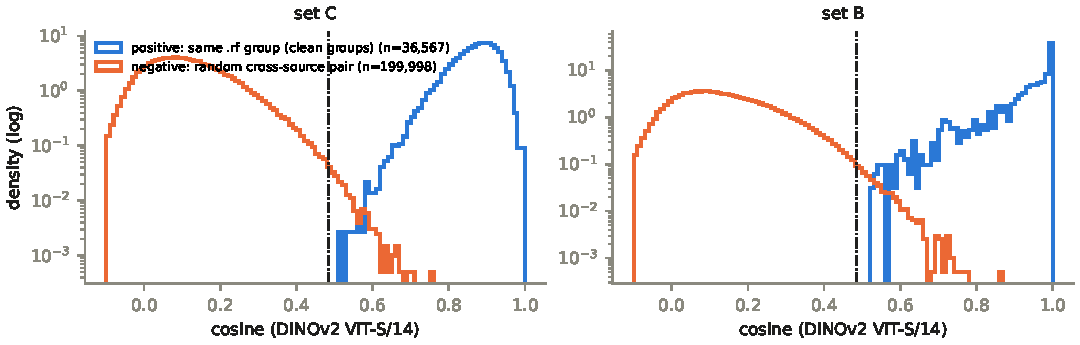
\includegraphics[width=\linewidth]{fig_cos_distribution.pdf}
\caption{DINOv2 cosine similarity of positive pairs (same augmentation
group) and random cross-source negatives in sources C and B; the
dash-dotted line is the cross-source threshold at precision 0.99.}
\label{fig:cosdist}
\end{figure}

\begin{figure}[!t]
\centering
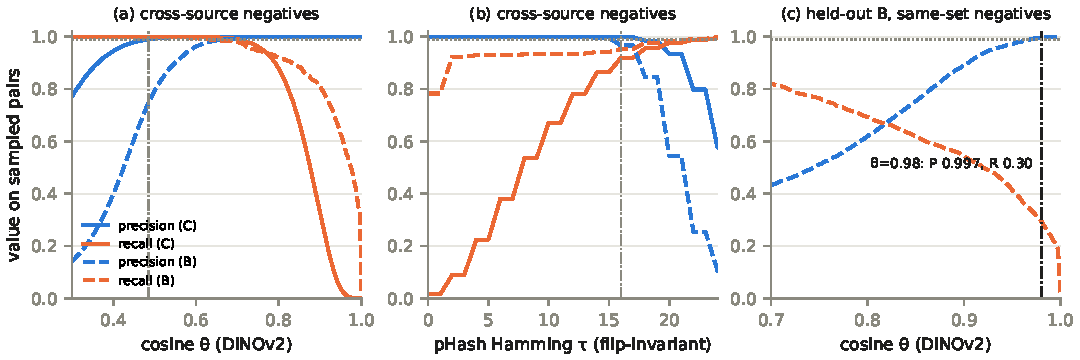
\includegraphics[width=\linewidth]{fig_calibration.pdf}
\caption{Precision and recall of the copy-level tier: (a) cosine and
(b) flip-invariant pHash against cross-source negatives; (c) cosine on
held-out B against same-set negatives, with the operating point
$\theta=0.98$.}
\label{fig:calibration}
\end{figure}

\subsection{Threshold sensitivity}
\label{sec:sensitivity}
Table~\ref{tab:threshold_sensitivity} applies four candidate rules to
the re-split of PPE-Unified (Section~\ref{sec:split}). Besides the
cross-source rule, an exhaustive cross-source search at false-positive
rate $\le10^{-7}$ gives $\theta=\ntsFprTheta$, $\tau=\ntsFprTau$; it
yields $\ntsFprGroups$ groups that no longer admit a 70/20/10 split
(largest class deviation $\ntsFprDev$ percentage points). At
$\theta=0.95$ the split is feasible but deviates by $\ntsNFDev$ points.
Only the operating point keeps the deviation at $\nvelDev$ points.
Sequence-level duplicates do not enter this trade-off: lowering
$\theta$ far enough to catch adjacent frames would merge unrelated
images of the same site, which is why tier~2b uses adjacency rather
than a similarity threshold.

\begin{table}[t]
\centering\footnotesize
\caption{Threshold sensitivity of the PPE-Unified v1.1 re-split. Groups = connected components of exact $\cup$ 2a($\theta,\tau$) $\cup$ 2b($k=2$); split by the group-aware stratified algorithm of v1 with background-aware counting (identical to v1 on singleton groups; seed 42, 70/20/10), on the corrected labels. Max.\ dev.\ = largest deviation of a class's box share from its target split share (v1: 0.07 pp). $\theta=0.98$ is the precision-conservative copy-level operating point; scene-level duplicates are handled by 2b, not by a threshold.}
\label{tab:threshold_sensitivity}
\begin{tabular}{lrrrrrl}
\toprule
Rule & $\theta$ & $\tau$ & Groups & Largest (\%) & Train/val/test & Max.\ dev.\ (pp) \\
\midrule
cross-source calibration, P$\ge$0.99 & 0.485 & 16 & 4 & 17{,}948 (99.98) & 0/17{,}950/1 & 80.0 (min-support FAIL) \\
FPR $\le 10^{-7}$, exhaustive cross-source & 0.8465 & 9 & 1{,}128 & 2{,}778 (15.48) & 10{,}356/3{,}532/4{,}063 & 57.65 \\
sensitivity & 0.95 & 4 & 1{,}499 & 1{,}915 (10.67) & 12{,}566/3{,}590/1{,}795 & 20.24 \\
\textbf{operating point (v1.1)} & 0.98 & 0 & 1{,}770 & 1{,}910 (10.64) & 12{,}566/3{,}590/1{,}795 & 4.12 \\
\bottomrule
\end{tabular}
\end{table}

\subsection{Audit results}
\label{sec:audit-results}
Table~\ref{tab:audit_v2} reports the audit. Source A has
$\nimgA$ images, B $\nimgB$ (in $\ngroupsB$ identifier groups,
multiplicity up to $\nmultMaxB\times$) and C $\nimgC$ (in $\ngroupsC$
groups, up to $\nmultMaxC\times$); SH17 has $\nimgSH$.

\emph{Exact tier.} B and C leak: $\nmultiB$ and $\nmultiC$ identifier
groups lie in more than one split, including $\nvtB$ and $\nvtC$
between validation and test. B additionally has $\nmdfiveCrossB$
byte-identical MD5 groups across splits. A, SH17 and PPE-Unified v1
pass.

\emph{Copy level.} At $\theta=\nopTheta$ tier~2a adds $\nextraCopyB$
cross-split pairs in B (+$\nextraCopyPctB$\% over the exact tier) and
$\nextraCopyC$ in C ($\nextraCopyXC\times$ the exact count), consistent with video
frames that carry distinct stems. A, clean at tier~1, has
$\ncopyA$ copy-level pairs ($\nleakImgCopyA$ images). PPE-Unified v1,
also clean at tier~1, has $\ncopyV$ pairs; $\nspanGroupsCopyV$ groups
($\nspanImgCopyV$ images) of exact $\cup$ 2a span splits. SH17 has no
copy-level pair at the operating point and $\ncopySHNF$ at
$\theta=0.95$.

\emph{Sequence level.} Tier~2b links $\nsceneV$ cross-split pairs in
PPE-Unified v1, $\nsceneB$ in B and $\nsceneC$ in C. Together with
tier~2a, $\nspanGroupsV$ groups ($\nspanImgV$ images) of PPE-Unified v1
span splits. SH17's official split has $\nsceneSH$ sequence-level
pairs; because tier~2b is a file-name rule without calibrated
precision, we report this count without classifying SH17 as leaky. For
A, sequential numeric file names chain every image into one 2b
component, so only A's pair counts are meaningful.

\emph{Across datasets.} The PPE-Unified v1 training split and the SH17
validation split, used for zero-shot evaluation in
Section~\ref{sec:e3}, share $\ncrossVSH$ pairs at every tier and
threshold, so that evaluation is not contaminated; the v1.1 training
split shares $\ncrossVelSHNinety$ copy-level pair with SH17, at
$\theta=0.90$ only.

\inputfloat{p}{\renewcommand{\arraystretch}{0.92}\begin{table*}[t]
\centering\footnotesize
\caption{Two-tier cross-split audit. Exact: same source ID or MD5. Copy level (2a): cosine $\ge\theta$ among FAISS top-5 neighbours or pHash $\le 0$ (flip-invariant); $\theta=0.98$ is the operating point, 0.95 and 0.90 are sensitivity. Scene level (2b): same file-name sequence, frame numbers within $\pm2$, no threshold. Pairs are counted across splits; +2a = 2a pairs not caught by the exact tier; groups = connected components of exact $\cup$ 2a $\cup$ 2b spanning more than one split (images).}
\label{tab:audit_v2}
\begin{tabular}{ll r rr rr rr rr}
\toprule
 & & & \multicolumn{2}{c}{$\theta=0.98$} & \multicolumn{2}{c}{$\theta=0.95$} & \multicolumn{2}{c}{$\theta=0.9$} & \multicolumn{2}{c}{2b scene} \\
\cmidrule(lr){4-5} \cmidrule(lr){6-7} \cmidrule(lr){8-9} \cmidrule(lr){10-11}
Dataset & Split pair & Exact & 2a & +2a & 2a & +2a & 2a & +2a & 2b & 2b-only \\
\midrule
PPE-U v1 & train-val & 0 & 2{,}912 & 2{,}912 & 6{,}508 & 6{,}508 & 18{,}774 & 18{,}774 & 7{,}155 & 6{,}420 \\
PPE-U v1 & train-test & 0 & 2{,}215 & 2{,}215 & 5{,}068 & 5{,}068 & 14{,}451 & 14{,}451 & 3{,}446 & 2{,}966 \\
PPE-U v1 & val-test & 0 & 932 & 932 & 2{,}217 & 2{,}217 & 5{,}681 & 5{,}681 & 1{,}377 & 1{,}149 \\
\multicolumn{11}{r}{\scriptsize groups spanning splits, exact only: 0 (0 img); exact$\cup$2a$\cup$2b at $\theta$ = 0.98, 0.95, 0.9: 666 (16{,}359) / 619 (16{,}553) / 523 (16{,}759)} \\
\midrule
PPE-U v1-fix & train-val & 0 & 2{,}912 & 2{,}912 & 6{,}508 & 6{,}508 & 18{,}774 & 18{,}774 & 7{,}155 & 6{,}420 \\
PPE-U v1-fix & train-test & 0 & 2{,}215 & 2{,}215 & 5{,}068 & 5{,}068 & 14{,}451 & 14{,}451 & 3{,}446 & 2{,}966 \\
PPE-U v1-fix & val-test & 0 & 932 & 932 & 2{,}217 & 2{,}217 & 5{,}681 & 5{,}681 & 1{,}377 & 1{,}149 \\
\multicolumn{11}{r}{\scriptsize groups spanning splits, exact only: 0 (0 img); exact$\cup$2a$\cup$2b at $\theta$ = 0.98, 0.95, 0.9: 666 (16{,}359) / 619 (16{,}553) / 523 (16{,}759)} \\
\midrule
PPE-U v1.1 & train-val & 0 & 0 & 0 & 883 & 883 & 7{,}145 & 7{,}145 & 0 & 0 \\
PPE-U v1.1 & train-test & 0 & 0 & 0 & 1{,}165 & 1{,}165 & 5{,}719 & 5{,}719 & 0 & 0 \\
PPE-U v1.1 & val-test & 0 & 0 & 0 & 170 & 170 & 1{,}214 & 1{,}214 & 0 & 0 \\
\multicolumn{11}{r}{\scriptsize groups spanning splits, exact only: 0 (0 img); exact$\cup$2a$\cup$2b at $\theta$ = 0.98, 0.95, 0.9: 0 (0) / 27 (6{,}437) / 53 (10{,}641)} \\
\midrule
SH17 & train-val & 0 & 0 & 0 & 9 & 9 & 127 & 127 & 1{,}660 & 1{,}626 \\
\multicolumn{11}{r}{\scriptsize groups spanning splits, exact only: 0 (0 img); exact$\cup$2a$\cup$2b at $\theta$ = 0.98, 0.95, 0.9: 595 (3{,}195) / 596 (3{,}223) / 589 (3{,}401)} \\
\midrule
A & train-test & 0 & 43 & 43 & 70 & 70 & 109 & 109 & 3 & 3 \\
\multicolumn{11}{r}{\scriptsize groups spanning splits, exact only: 0 (0 img); exact$\cup$2a$\cup$2b at $\theta$ = 0.98, 0.95, 0.9: 1 (7{,}035) / 1 (7{,}035) / 1 (7{,}035)} \\
\midrule
B & train-val & 2{,}154 & 1{,}712 & 704 & 2{,}952 & 1{,}874 & 6{,}120 & 4{,}975 & 8{,}420 & 4{,}952 \\
B & train-test & 1{,}088 & 938 & 389 & 1{,}539 & 950 & 3{,}884 & 3{,}265 & 4{,}247 & 2{,}491 \\
B & val-test & 331 & 269 & 117 & 437 & 273 & 1{,}170 & 990 & 1{,}226 & 719 \\
\multicolumn{11}{r}{\scriptsize groups spanning splits, exact only: 573 (2{,}441 img); exact$\cup$2a$\cup$2b at $\theta$ = 0.98, 0.95, 0.9: 372 (4{,}719) / 353 (4{,}745) / 280 (4{,}811)} \\
\midrule
C & train-val & 1{,}491 & 7{,}207 & 7{,}158 & 13{,}094 & 13{,}010 & 50{,}182 & 49{,}994 & 25{,}011 & 20{,}671 \\
C & train-test & 810 & 3{,}804 & 3{,}763 & 8{,}330 & 8{,}271 & 39{,}853 & 39{,}750 & 12{,}576 & 9{,}991 \\
C & val-test & 64 & 5{,}440 & 5{,}383 & 7{,}899 & 7{,}842 & 11{,}670 & 11{,}611 & 1{,}155 & 442 \\
\multicolumn{11}{r}{\scriptsize groups spanning splits, exact only: 831 (3{,}196 img); exact$\cup$2a$\cup$2b at $\theta$ = 0.98, 0.95, 0.9: 157 (29{,}749) / 137 (29{,}897) / 104 (30{,}118)} \\
\midrule
\multicolumn{2}{l}{PPE-U v1-train vs SH17-val} & 0 & 0 & 0 & 0 & 0 & 0 & 0 & -- & -- \\
\multicolumn{2}{l}{PPE-U v1.1-train vs SH17-val} & 0 & 0 & 0 & 0 & 0 & 1 & 1 & -- & -- \\
\bottomrule
\end{tabular}
\end{table*}}

\subsection{Errata to PPE-Unified v1 and to the earlier study}
\label{sec:errata}
The audit changes statements made in the earlier version of this
study and in the v1 release; we list them here.
(i) \emph{PPE-Unified v1 is not leak-free.} It passes the exact tier
but holds $\ncopyV$ copy-level and $\nsceneV$ sequence-level
cross-split pairs (above), inherited from source C's video frames.
Baseline scores measured on v1 (E1, Section~\ref{sec:e1}) are
therefore reported as published reference values, and v1.1 replaces
v1 (Section~\ref{sec:dataset}).
(ii) \emph{Source statistics.} The earlier audit table reported
$\nvFourImgB$ images for B and $\nvFourImgC$ for C; the exports hold $\nimgB$ and
$\nimgC$ images ($\ngroupsC$ is C's number of identifier groups), and
A holds $\nimgA$. Augmentation multiplicities are up to
$\nmultMaxB\times$ for B and $\nmultMaxC\times$ for C, not
${\sim}3\times$ and $3$--$16\times$.
(iii) \emph{Validation--test overlap} ($\nvtB$ groups in B, $\nvtC$ in
C) was not counted, nor were B's $\nmdfiveCrossB$ cross-split MD5
groups.
(iv) \emph{The clean arms of the leaky-versus-clean experiment still
leak.} They were grouped by identifier only and keep $\narmBExCos$
(B) and $\narmCExCos$ (C) cross-split pairs with cosine
$\ge\nopTheta$; the C arm keeps more than C's original split
($\narmCOrigCos$), because shuffling identifier groups scatters video
frames over all three splits. The inflation measured against these
arms ($\neTwoMin$ to $\neTwoMax$ mAP@50 points) is therefore a lower
bound.
(v) The validator released with v1 implemented two of its eight
checks more weakly than described (pair consistency and full decoding);
it has been brought up to the description
(Section~\ref{sec:validation}), which exposed $\nlabelFixes$ label
errors that are corrected in v1.1.

%% ============================================================
\section{The PPE-Unified v1.1 benchmark}
\label{sec:dataset}

\subsection{Sources, taxonomy and construction}
PPE-Unified merges three sources released under CC~BY~4.0: a
helmet-focused collection (A), a five-pair compliance dataset (B) and
a ten-class PPE dataset (C). Labels are mapped to twelve classes forming
six compliance--violation pairs (\emph{helmet}\slash\emph{no\_helmet},
\emph{vest}\slash\emph{no\_vest}, \emph{gloves}\slash\emph{no\_gloves},
\emph{goggles}\slash\emph{no\_goggles}, \emph{boots}\slash\emph{no\_boots},
\emph{mask}\slash\emph{no\_mask}); naming variants are resolved
(\emph{head}$\to$\emph{no\_helmet}) and out-of-scope classes dropped.
SH17 is held out, both because its licence forbids redistribution and
to keep an out-of-distribution test set. The scripted pipeline
(Fig.~\ref{fig:pipeline}) groups variants by source identifier,
removes cross-source MD5 duplicates, re-maps classes, sub-samples
over-represented helmet-only imagery, caps background images at 10\%,
letterboxes all images to $640\times640$, splits, and validates. The
corpus has $\nimgV$ images and $\nvelBoxes$ boxes after the label
corrections.

\begin{figure}[!t]
\centering
\includegraphics[width=0.7\linewidth]{fig_pipeline.pdf}
\caption{The PPE-Unified v1.1 construction pipeline (image counts of
the source exports). Every stage is scripted; the last stage re-runs
the eight-point validation after any change, and a failure blocks
release. v1 differed in step~5, which grouped by source identifier
only.}
\label{fig:pipeline}
\end{figure}

\subsection{Near-duplicate-aware group split}
\label{sec:split}
v1 grouped images by source identifier only ($\nvOneGroups$ groups,
all singletons after de-duplication). v1.1 groups them by the
connected components of exact $\cup$ 2a $\cup$ 2b at the operating
point ($\nvelEdgesCos$ cosine, $\nvelEdgesPh$ pHash and
$\nvelEdgesScene$ sequence links), giving $\nvelGroups$ groups; the
largest holds $\nvelLargest$ images ($\nvelLargestPct$\%). Groups are
assigned by the v1 algorithm: a greedy pass in decreasing order of
rarity-weighted class content that minimises a quadratic penalty on
the deviation of every class proportion from its 70/20/10 target, with
per-process-independent iteration order and retries over fixed seeds.
We extend it with background-aware counting, which balances label-free
images per image rather than per group. On singleton groups the
extended algorithm reproduces the v1 split for $\ncompatPct$\% of the
images, so the two releases differ only through the grouping.

The result has $\nvelTrain$, $\nvelVal$ and $\nvelTest$ train,
validation and test images ($\nvelTrainPct$, $\nvelValPct$ and $\nvelTestPct$\%), of which
$\nvelBgTrain$, $\nvelBgVal$ and $\nvelBgTest$ are background images. Large groups cost class balance: the largest
deviation of a class share from its target is $\nvelDev$ percentage
points, against $\nvOneDev$ in v1; every class still meets its minimum
support. At the operating point v1.1 has zero cross-split pairs at
every tier. At the sensitivity thresholds it keeps $\ncopyVelNF$ pairs
at $\theta=0.95$ ($\nleakImgCopyVelNF$ images) and $\ncopyVelNinety$ at
$\theta=0.90$ (Table~\ref{tab:audit_v2}). The $\nlabelFixes$ label
corrections ($\nlabelFixClip$ boxes clipped to the image,
$\nlabelFixDrop$ contradictory boxes removed) are applied to one
corrected pool from which two releases are cut: \emph{v1-fix} keeps the
v1 split and \emph{v1.1} the new one. Both ship a per-file manifest, a
corrections log and a SHA256SUMS file.

\subsection{Schema-driven eight-point validation}
\label{sec:validation}
Every release must pass eight checks:
(1) class IDs in range and class names matching the schema;
(2) boxes normalised and inside the image, one label file per image;
(3) no box labelled both as compliance and as violation of one pair
(IoU $\ge0.8$), and every pair present in every split;
(4) uniform image size, where the schema declares one;
(5) zero cross-split leakage at the group key, MD5, tier~2a
(exhaustive search) and tier~2b;
(6) every image fully decodable;
(7) minimum per-class support in each split;
(8) background share within tolerance across splits.
The validator is one program. Everything dataset-specific---format
(YOLO or COCO), class list, compliance--violation pairs, split names
and targets, the group key, the thresholds and the support
minima---lives in a schema file of about twenty lines; a check whose
input the schema does not declare reports N/A rather than PASS.

Table~\ref{tab:generality} runs the same validator code on four
datasets. PPE-Unified v1.1 passes 8/8; v1-fix fails only check~5, with
$\nvalVfixCopy$ copy-level and $\nvalVfixScene$ sequence-level
cross-split pairs (the exhaustive count exceeds the top-$\nopTopk$
audit count of Table~\ref{tab:audit_v2}). On Virtual KITTI~2
($\nimgVk$ frames split 70/20/10 at random, as is common) it reports
$\npassVk$/$\nfailVk$/$\nnaVk$ PASS/FAIL/N/A, with $\ncopyVkVal$
copy-level and $\nsceneVkVal$ sequence-level leaks. On VIRAT with
IARPA DIVA boxes ($\nimgVi$ frames, official clip-level split) it
reports $\npassVi$/$\nfailVi$/$\nnaVi$, including $\ncopyViVal$
copy-level pairs across the official split. Neither dataset required a
code change.

\inputfloat{tp}{\begin{table*}[t]
\centering\footnotesize
\caption{Eight-point validation with one unchanged, schema-driven validator on PPE and non-PPE data. Leakage cell: (groups or MD5 across splits / copy-level 2a pairs, any cosine $\ge0.98$ or pHash $=0$ / scene-level 2b pairs). N/A = the schema declares nothing to check. $^a$Virtual KITTI~2 clone, Camera~0, 5 scenes, frames shuffled 70/20/10 (common practice); $^b$VIRAT ground video, IARPA DIVA boxes, 1 frame/s, official train/validate split by clip.}
\label{tab:generality}
\begin{tabular}{lllll}
\toprule
Check & PPE-U v1.1 & PPE-U v1-fix & VKITTI2$^a$ & VIRAT-DIVA$^b$ \\
Images & 17{,}951 & 17{,}951 & 2{,}126 & 1{,}227 \\
\midrule
1 Class IDs & PASS & PASS & PASS & PASS \\
2 Boxes / pairing & PASS & PASS & FAIL (2 bad) & PASS \\
3 Compl.--viol.\ pairs & PASS & PASS & N/A (no pairs) & N/A (no pairs) \\
4 Uniform size & PASS & PASS & PASS & N/A (mixed sizes) \\
5 Leakage (ID, MD5, 2a, 2b) & PASS (0/0/0) & FAIL (0/12{,}582/11{,}978) & FAIL (0/2{,}221/1{,}961) & FAIL (0/44{,}109/0) \\
6 Corrupt images & PASS (17{,}951 dec.) & PASS (17{,}951 dec.) & PASS (2{,}126 dec.) & PASS (1{,}227 dec.) \\
7 Min.\ support & PASS & PASS & FAIL (2 viol.) & FAIL (3 viol.) \\
8 Background share & PASS (0.3 pp) & PASS (0.1 pp) & FAIL (5.0 pp) & N/A (no bg.\ images) \\
\midrule
PASS / FAIL / N/A & 8 / 0 / 0 & 7 / 1 / 0 & 3 / 4 / 1 & 3 / 2 / 3 \\
\bottomrule
\end{tabular}
\end{table*}}

%% ============================================================
\section{Experimental setup}
\label{sec:experiments}

\subsection{Architecture families and protocol}
\textbf{CNN.} YOLO26s \citep{ultralytics_yolo26} and Faster R-CNN
R50-FPN \citep{ren2015faster} are trained as detectors; VGG16 and
ResNet50 as compliance classifiers on ground-truth crops.
\textbf{Recurrent.} GRU, LSTM and their bidirectional and stacked
variants read each $128\times128$ crop as a 128-step sequence of row
vectors. \textbf{Transformer.} RT-DETR-L \citep{zhao2024rtdetr} is
trained as a detector; ViT-B/16 and ViT-S/16, ImageNet-pretrained
\citep{deng2009imagenet}, are fine-tuned on crops. Every model has a
screening HPO stage on the validation split; the test split is used
once per final model. Detectors report mAP@50 and mAP@50--95.
Training uses Kaggle T4 instances with checkpoint-resume across
12-hour sessions.

\subsection{Experiments}
\label{sec:e-list}
\textbf{E1 (reference baselines).} All nine models on PPE-Unified v1,
as published in the earlier version. Because v1 leaks at the
perceptual tier (Section~\ref{sec:errata}), E1 values are reference
values, not verified-split estimates.

\textbf{E2$'$ (v1 versus v1.1).} YOLO26s and RT-DETR-L with the HPO
configuration of E1 (30 epochs, $640$ px, repeat-factor sampling on
train) on v1-fix and on v1.1. Both use the same corrected images and
labels, so the comparison isolates the split. YOLO26s runs seeds 0
and 1 per split; RT-DETR-L runs seed 0.

\textbf{E2$''$ (leaked versus clean test images).} Inference only: the
v1-fix models of E2$'$ on subsets of the v1 test split defined by the
audit (Section~\ref{sec:e2pp}).

\textbf{E2-B (four arms of source B).} YOLO26s (15
epochs, $640$ px) on four splits of the same B pool
(Table~\ref{tab:arms}): the authors' \emph{original} split; the
identifier-grouped \emph{clean-exact} split of the earlier study; a
class-balanced variant of it (\emph{clean-exact-balanced}); and
\emph{clean2}, grouped by exact $\cup$ 2a $\cup$ 2b and balanced.
Seeds 42 and 0 for the two new arms. RT-DETR-L was trained on the
original and clean-exact arms in the earlier study; it was not run on
the two new arms.

\textbf{E2-C (leave-one-sequence-out on source C).} Grouping C by
exact $\cup$ 2a $\cup$ 2b leaves $\narmCTwoGroups$ groups, and the
$\nseqN$ largest are video sequences holding $\nseqPct$\% of the
images. A sequence must stay in one split, and the sequences hold most
boxes of several classes (Section~\ref{sec:loso-res}), so no
class-balanced 70/20/10 split exists. We therefore hold out one
sequence per fold: train on the other three and on all images outside
the sequences, test on the held-out sequence. All four folds have zero
train--test pairs at every tier (Table~\ref{tab:loso}). The protocol
has no validation split: YOLO26s (seed 42) trains for the fixed E2
epoch count, is evaluated at the last checkpoint, and a class with no
test box in a fold is reported N/A. The folds are released; detectors
were not trained on them for this paper.

\textbf{E3 (cross-dataset).} The best E1 detectors are evaluated
zero-shot on SH17 on the four shared classes (helmet, vest, gloves,
mask); only the remapping script is released.
\textbf{E4--E6.} Seed robustness, repeat-factor sampling and
resolution ablations of the earlier version, on v1.

\begin{table}[t]
\centering
\caption{E2-B: four splits of the same source-B pool. Groups and
largest group size of the grouping key; Dev.\ = largest deviation of a
class share from its split target (pp); cross-split pairs by tier
(cosine at $\theta=0.98$). mAP@50 on each arm's test split; original
and clean-exact are the earlier E2 runs (seed 42), the other two arms
the mean of seeds 42 and 0 (YOLO26s, two seeds). n.r.\ = not run.}
\label{tab:arms}
\footnotesize
\setlength{\tabcolsep}{3pt}
\begin{tabular}{lrrrrrrrcc}
\toprule
Arm & Groups & Largest & Dev. & Exact & Cos & pHash & 2b & YOLO26s & RT-DETR-L \\
\midrule
original & \narmBOrigGroups & \narmBOrigLargest & \narmBOrigDev & \narmBOrigExact & \narmBOrigCos & \narmBOrigPh & \narmBOrigScene & \neTwoYoloBLeaky & \neTwoDetrBLeaky \\
clean-exact & \narmBExGroups & \narmBExLargest & \narmBExDev & \narmBExExact & \narmBExCos & \narmBExPh & \narmBExScene & \neTwoYoloBClean & \neTwoDetrBClean \\
clean-exact-bal. & \narmBExBalGroups & \narmBExBalLargest & \narmBExBalDev & \narmBExBalExact & \narmBExBalCos & \narmBExBalPh & \narmBExBalScene & \ntTwoBExBalYolo & \ntTwoBExBalDetr \\
clean2 & \narmBTwoGroups & \narmBTwoLargest & \narmBTwoDev & \narmBTwoExact & \narmBTwoCos & \narmBTwoPh & \narmBTwoScene & \ntTwoBTwoYolo & \ntTwoBTwoDetr \\
\bottomrule
\end{tabular}
\end{table}

%% ============================================================
\section{Results and discussion}
\label{sec:results}

\subsection{Inflation on PPE-Unified: v1 versus v1.1}
\label{sec:ppeu-infl}
Table~\ref{tab:t4} compares the same detectors on v1-fix and v1.1.
YOLO26s reaches \ntFourYoloFix{} mAP@50 on v1-fix
(\ntFourYoloFixN{} seeds) and \ntFourYoloVel{} on v1.1
(\ntFourYoloVelN{} seeds), a difference of \ntFourYoloInfl{}
points; RT-DETR-L (\ntFourDetrFixN{} seed per split) reaches
\ntFourDetrFix{} and \ntFourDetrVel{}, a difference of \ntFourDetrInfl{}
points. The difference is
not leakage alone: v1.1 holds out whole near-duplicate groups,
including long video sequences, so its test split also asks for
generalisation to unseen scenes. The gap therefore measures how much
the v1 split overstates performance on unseen scenes, not leakage in
isolation.

\begin{table}[t]
\centering
\caption{E2$'$: YOLO26s and RT-DETR-L on v1-fix (v1 split) and v1.1
(near-duplicate-aware split) of the same corrected images; test
mAP, mean over \ntFourYoloFixN{} seeds (YOLO26s, seeds 0 and 1) and
\ntFourDetrFixN{} seed (RT-DETR-L, seed 0) per split. $\Delta$ =
v1-fix $-$ v1.1 in points.}
\label{tab:t4}
\footnotesize
\begin{tabular}{lcccccc}
\toprule
 & \multicolumn{2}{c}{v1-fix} & \multicolumn{2}{c}{v1.1} & \multicolumn{2}{c}{$\Delta$} \\
\cmidrule(lr){2-3}\cmidrule(lr){4-5}\cmidrule(lr){6-7}
Detector & @50 & @50--95 & @50 & @50--95 & @50 & @50--95 \\
\midrule
YOLO26s   & \ntFourYoloFix & \ntFourYoloFixHi & \ntFourYoloVel & \ntFourYoloVelHi & \ntFourYoloInfl & \ntFourYoloInflHi \\
RT-DETR-L & \ntFourDetrFix & \ntFourDetrFixHi & \ntFourDetrVel & \ntFourDetrVelHi & \ntFourDetrInfl & \ntFourDetrInflHi \\
\bottomrule
\end{tabular}
\end{table}

\subsection{Same model, leaked versus clean test images (E2$''$)}
\label{sec:e2pp}
The v1 versus v1.1 comparison changes the test split as well as the
leakage, so it cannot say how much of the gap is leakage and how much
is a harder test set. E2$''$ holds model and test split fixed. We take
the v1-fix models of E2$'$ (YOLO26s seeds 0 and 1, RT-DETR-L seed 0;
inference only) and split the v1 test set in two ways
(Table~\ref{tab:e2pp}). \emph{Group-leaked} images belong to a
near-duplicate group (exact $\cup$ 2a $\cup$ 2b) that also has training
or validation images; this covers $\neppGrpImg$ of the $\neppFullImg$
test images ($\neppGrpPct$\%), leaving $\neppGrpCleanImg$ group-clean
images. \emph{Copy-leaked} images have a direct exact or copy-level
partner in training or validation ($\neppCpImg$ images,
$\neppCpPct$\%). Each pair of subsets is compared on the classes with
at least $\neppMinGt$ boxes in both ($\neppGrpNCls$ and $\neppCpNCls$
classes), with $\neppBoot$ bootstrap resamples over images. On the full
test split the metric reproduces Ultralytics validation
($\neppYoloAVal$, $\neppYoloBVal$ and $\neppDetrVal$ mAP@50).

All $\neppNModels$ models score $\neppGrpDeltaMin$ to
$\neppGrpDeltaMax$ mAP@50 points higher on group-leaked than on
group-clean images, and every 95\% interval excludes zero. A direct copy
in the training split adds nothing beyond that: copy-leaked and other
test images differ by $\neppCpDeltaMin$ to $\neppCpDeltaMax$ points,
with intervals that include zero. At mAP@50--95 the group effect is
smaller and its interval excludes zero for RT-DETR-L only
(Table~\ref{tab:e2pp}). The benefit of leakage in v1 therefore comes
from sharing a scene or sequence with the training data, which most
test images do, rather than from exact or near copies. Identifier, hash
and copy-level checks are necessary to find the leak, but they do not
bound its effect; sequence-aware grouping does, which is why v1.1 holds
out whole groups.

Tier~2b dominates because of how PPE imagery is acquired. Much of it is
CCTV or handheld video, and consecutive frames of one camera show the
same background, workers and equipment under small changes of pose and
position. Such frames rarely reach the copy-level threshold, yet a
detector trained on some of them has, in effect, seen the scene of the
rest. In v1 this channel is the larger one: the audit finds
$\nsceneV$ sequence-level against $\ncopyV$ copy-level cross-split
pairs, and the groups they form reach the training or validation split
for $\neppGrpPct$\% of the test images. The copy-level comparison is
nested inside this: every copy-leaked image is also group-leaked, and
the images it is compared with are group-leaked too except for the
$\neppGrpCleanImg$ group-clean ones, so the comparison asks whether a
direct copy adds anything once the scene
is shared. At this sample size it does not.

The comparison has three measured limits. The group-clean subset is
small ($\neppGrpCleanImg$ images, $\neppGrpCleanBox$ boxes, compared on
$\neppGrpNCls$ of the twelve classes) and is not a random sample:
images whose group lies wholly in the test split may differ in source
and difficulty from the rest, so E2$''$ separates the leakage effect
from the choice of split but not from every difference between images.
The \emph{no\_boots} class has four test boxes; it is excluded from both
paired comparisons, and on the full split the interval of RT-DETR-L
is asymmetric about the point estimate, as expected when resamples drop
or repeat these few boxes. And after
de-duplication the copy-leaked subset is small ($\neppCpImg$ images,
$\neppCpBox$ boxes), so its intervals span $\neppYoloBCpDeltaLo$ to
$\neppDetrCpDeltaUp$ points: a copy effect of a few points in either
direction is compatible with the data. E2$''$ complements the
re-training comparison of Section~\ref{sec:ppeu-infl}.

\begin{table}[tp]
\centering\footnotesize
\caption{E2$''$: the same v1-fix models on subsets of the v1 test split. Group-leaked: the image's near-duplicate group (exact $\cup$ 2a $\cup$ 2b, operating point) also has train or validation images. Copy-leaked: the image itself has an exact or copy-level (2a) partner in train or validation. Full test: all classes (equals Ultralytics val); each leaked/clean pair: mean over the classes with at least 10 boxes in both subsets. 95\% bootstrap CI over images (1{,}000 resamples); $\Delta$ = leaked $-$ clean, in points.}
\label{tab:e2pp}
\setlength{\tabcolsep}{3pt}
\begin{tabular}{llrrcc}
\toprule
Model & Test subset & Images & Boxes & mAP@50 [95\% CI] & mAP@50--95 [95\% CI] \\
\midrule
yolo26s s0 & full test & 1{,}795 & 5{,}114 & 0.795 [0.780, 0.810] & 0.503 [0.491, 0.518] \\
 & group-leaked & 1{,}677 & 4{,}832 & 0.913 [0.901, 0.925] & 0.588 [0.574, 0.603] \\
 & group-clean & 118 & 282 & 0.858 [0.810, 0.908] & 0.562 [0.518, 0.618] \\
 & $\Delta$ & & & $+5.5$ [$+0.5$, $+10.5$] & $+2.5$ [$-2.9$, $+7.5$] \\
 & copy-leaked & 289 & 462 & 0.886 [0.850, 0.920] & 0.580 [0.548, 0.621] \\
 & not copy-leaked & 1{,}506 & 4{,}652 & 0.893 [0.877, 0.909] & 0.577 [0.562, 0.594] \\
 & $\Delta$ & & & $-0.7$ [$-4.5$, $+3.2$] & $+0.4$ [$-3.2$, $+4.5$] \\
\midrule
yolo26s s1 & full test & 1{,}795 & 5{,}114 & 0.800 [0.786, 0.819] & 0.507 [0.497, 0.522] \\
 & group-leaked & 1{,}677 & 4{,}832 & 0.915 [0.903, 0.927] & 0.590 [0.578, 0.605] \\
 & group-clean & 118 & 282 & 0.833 [0.783, 0.889] & 0.544 [0.506, 0.595] \\
 & $\Delta$ & & & $+8.2$ [$+2.4$, $+13.5$] & $+4.6$ [$-0.3$, $+8.7$] \\
 & copy-leaked & 289 & 462 & 0.884 [0.846, 0.919] & 0.589 [0.554, 0.630] \\
 & not copy-leaked & 1{,}506 & 4{,}652 & 0.901 [0.886, 0.915] & 0.581 [0.568, 0.597] \\
 & $\Delta$ & & & $-1.7$ [$-5.9$, $+2.1$] & $+0.7$ [$-3.6$, $+4.9$] \\
\midrule
rtdetr-l s0 & full test & 1{,}795 & 5{,}114 & 0.781 [0.765, 0.832] & 0.479 [0.468, 0.509] \\
 & group-leaked & 1{,}677 & 4{,}832 & 0.902 [0.891, 0.915] & 0.562 [0.549, 0.579] \\
 & group-clean & 118 & 282 & 0.800 [0.747, 0.863] & 0.502 [0.458, 0.562] \\
 & $\Delta$ & & & $+10.3$ [$+3.9$, $+15.8$] & $+6.0$ [$+0.1$, $+10.8$] \\
 & copy-leaked & 289 & 462 & 0.874 [0.833, 0.915] & 0.562 [0.527, 0.606] \\
 & not copy-leaked & 1{,}506 & 4{,}652 & 0.875 [0.859, 0.894] & 0.549 [0.534, 0.567] \\
 & $\Delta$ & & & $-0.1$ [$-4.5$, $+4.4$] & $+1.3$ [$-2.6$, $+5.9$] \\
\bottomrule
\end{tabular}
\end{table}


\subsection{Source B: four split arms}
\label{sec:arms-res}
The earlier experiment trained each detector on B's original split and
on the clean-exact split: leakage inflated test mAP@50 by
$\neTwoYoloBInfl$ points (YOLO26s) and $\neTwoDetrBInfl$ (RT-DETR-L),
and on C by $\neTwoYoloCInfl$ and $\neTwoDetrCInfl$. Since the
clean-exact arms keep copy-level and sequence-level pairs
(Table~\ref{tab:arms}), these are lower bounds. Grouping B by all
three tiers collapses $\narmBExGroups$ identifier groups into
$\narmBTwoGroups$, the largest with $\narmBTwoLargest$ images, yet a
class-balanced split remains feasible (deviation $\narmBTwoDev$ pp).

For YOLO26s (Table~\ref{tab:arms}; mean of two seeds, largest seed
standard deviation $\ntTwoBSeedSdYolo$) the clean2 arm scores
$\ntTwoBTwoYolo$ mAP@50, so the original split overstates it by
$\ntTwoBInflYolo$ points, against the $\neTwoYoloBInfl$ measured
against the clean-exact arm. The intermediate arm decomposes the
difference: balancing the exact-grouped split lowers the score by
$\ntTwoBStepBalYolo$ points (to $\ntTwoBExBalYolo$), and adding the
perceptual tiers to the grouping lowers it by a further
$\ntTwoBStepTwoYolo$. The arms differ in their test images, so each
step mixes the removal of near-duplicates with a change of test
composition; the clean2 arm is the only one with no cross-split pair
at any tier. RT-DETR-L was not run on the two new arms, so the
inflation over clean2 is measured for YOLO26s only.

\subsection{Source C: no clean balanced split exists}
\label{sec:loso-res}
For C the three-tier grouping is decisive. Its $\nseqN$ largest groups
are video sequences holding $\nseqPct$\% of the images, and they hold
most boxes of several classes: one sequence holds $\nseqPPnoglove$\%
of all \emph{no\_glove} boxes and $\nseqPPglove$\% of \emph{glove}
boxes, another $\nseqKpGoggles$\% of \emph{goggles}, a third
$\nseqPackNoGoggles$\% of \emph{no\_goggles}. Because each sequence must
lie in one split, the best balanced assignment still deviates by
$\nseqDev$ percentage points from the class targets (tolerance
$\pm\nseqTarget$). A clean 70/20/10 split of C with balanced classes
does not exist; any split that reports balanced classes on C must
cross sequences. We report this as a finding about the dataset and
define leave-one-sequence-out folds for C (Table~\ref{tab:loso}). Each
fold can test only the classes present in its held-out sequence;
\emph{helmet} and \emph{no\_helmet} occur only outside the sequences
and are not testable in any fold.

\begin{table}[t]
\centering
\caption{E2-C: leave-one-sequence-out folds on source C (protocol:
YOLO26s, seed 42, fixed epochs, last checkpoint; not run for this
paper). All folds have zero train--test pairs at every tier;
cos$\ge$0.95 pairs are given for information. Evaluable classes have
at least one box in the held-out sequence.}
\label{tab:loso}
\footnotesize
\setlength{\tabcolsep}{4pt}
\begin{tabular}{clrrlr}
\toprule
Fold & Held-out seq. & Train & Test & Evaluable classes & cos$\ge$0.95 \\
\midrule
0 & \nlosoASeq & \nlosoATrain & \nlosoATest & \nlosoAEval & \nlosoACosNF \\
1 & \nlosoBSeq & \nlosoBTrain & \nlosoBTest & \nlosoBEval & \nlosoBCosNF \\
2 & \nlosoCSeq & \nlosoCTrain & \nlosoCTest & \nlosoCEval & \nlosoCCosNF \\
3 & \nlosoDSeq & \nlosoDTrain & \nlosoDTest & \parbox[t]{3.2cm}{\raggedright\nlosoDEval} & \nlosoDCosNF \\
\bottomrule
\end{tabular}
\end{table}

\subsection{Reference baselines (E1) and ablations on v1}
\label{sec:e1}
Table~\ref{tab:e1} reports the E1 baselines on v1. Among detectors,
RT-DETR-L reaches $\neOneDetr$ mAP@50 at $\neOneDetrMs$\,ms per image
and YOLO26s $\neOneYolo$ at $\neOneYoloMs$\,ms ($\neOneSpeedup\times$
faster); Faster R-CNN trails ($\neOneFrcnn$). Among crop classifiers
ViT-B/16 leads (accuracy $\neOneVitBAcc$, macro-F1 $\neOneVitBFone$),
ViT-S/16 has the best worst-class F1 ($\neOneVitSWorst$), and the best
recurrent model reaches macro-F1 $\neOneGruFone$, the cost of forcing a
sequence model onto a spatial task. Both detectors agree on the hard
classes (Table~\ref{tab:perclass}): \emph{no\_vest} and
\emph{no\_boots}, the latter with four test boxes. These values were
measured on the v1 split and share its leakage; the v1-fix runs of
E2$'$, with the same configuration, give comparable numbers
(Table~\ref{tab:t4}), while the v1.1 runs give the verified estimate.

Seed variation is small: four YOLO26s seeds give $\neFourMean\pm\neFourStd$
mAP@50 (E4). Repeat-factor sampling moves overall mAP@50 from
$\neFiveOff$ to $\neFiveOn$, with the gain concentrated on rare classes
(E5). Letterboxing source C from 416 to 640 px raises mAP@50 by
$\neSixGain$ points on the C subset (E6), so the normalisation is not
harmful.

\begin{table}[t]
\centering
\caption{E1 reference baselines on PPE-Unified v1 (test split; HPO on
validation), as published. Detectors: mAP@50, mAP@50--95, latency.
Classifiers (ground-truth crops): accuracy, macro-F1, worst-class F1.
v1 shares near-duplicates across splits (Section~\ref{sec:errata}).}
\label{tab:e1}
\footnotesize
\setlength{\tabcolsep}{4pt}
\begin{tabular}{llccc}
\toprule
Family & Model & mAP@50 & mAP@50--95 & ms/img \\
\midrule
CNN & YOLO26s & \neOneYolo & \neOneYoloHi & \neOneYoloMs \\
CNN & Faster R-CNN R50-FPN & \neOneFrcnn & \neOneFrcnnHi & \neOneFrcnnMs \\
Transf. & RT-DETR-L & \neOneDetr & \neOneDetrHi & \neOneDetrMs \\
\midrule
 & & Accuracy & Macro-F1 & Worst-F1 \\
\midrule
CNN & ResNet50 (crops) & \neOneRnAcc & \neOneRnFone & \neOneRnWorst \\
CNN & VGG16 (crops) & \neOneVggAcc & \neOneVggFone & \neOneVggWorst \\
RNN & GRU-256 (best RNN) & \neOneGruAcc & \neOneGruFone & \neOneGruWorst \\
Transf. & ViT-B/16 & \neOneVitBAcc & \neOneVitBFone & \neOneVitBWorst \\
Transf. & ViT-S/16 & \neOneVitSAcc & \neOneVitSFone & \neOneVitSWorst \\
\bottomrule
\end{tabular}
\end{table}

\begin{table}[t]
\centering
\caption{Per-class AP@50 on the PPE-Unified v1 test split (E1).}
\label{tab:perclass}
\footnotesize
\setlength{\tabcolsep}{4pt}
% Generated by scripts/make_appendix_tables.py from results/extended -- do not edit by hand.
\begin{tabular}{lrcc@{\hskip 0.8em}lrcc}
\toprule
Class & Boxes & YOLO26s & RT-DETR & Class & Boxes & YOLO26s & RT-DETR \\
\midrule
helmet & 1{,}649 & 0.952 & 0.946 & goggles & 368 & 0.889 & 0.928 \\
no\_helmet & 827 & 0.917 & 0.934 & no\_goggles & 386 & 0.830 & 0.837 \\
vest & 290 & 0.907 & 0.918 & boots & 111 & 0.899 & 0.896 \\
no\_vest & 112 & \textbf{0.514} & \textbf{0.537} & no\_boots & 4 & \textbf{0.012} & \textbf{0.061} \\
gloves & 501 & 0.803 & 0.800 & mask & 118 & 0.939 & 0.912 \\
no\_gloves & 616 & 0.836 & 0.839 & no\_mask & 132 & 0.970 & 0.942 \\
\bottomrule
\end{tabular}

\end{table}

\subsection{Cross-dataset generalisation (E3)}
\label{sec:e3}
Zero-shot on SH17's four shared classes, YOLO26s falls from
$\neThreeYoloIn$ to $\neThreeYolo$ mAP@50 ($-\neThreeYoloDrop$\%) and
RT-DETR-L from $\neThreeDetrIn$ to $\neThreeDetr$
($-\neThreeDetrDrop$\%), the latter driven by helmet
($\neThreeDetrHelmet$) and vest ($\neThreeDetrVest$)
(Table~\ref{tab:e3}). The PPE-Unified v1 training split and SH17 share
no pair at any audited tier or threshold (Section~\ref{sec:audit-results}),
so the comparison is not contaminated by near-duplicates. Three factors compound: a
genuine domain gap (diverse industrial settings at high native
resolution versus construction imagery at $640\times640$, which
shrinks small objects \citep{cheng2023small}); label-definition
mismatch (SH17 annotates gloves per hand and masks more narrowly); and
the absence of any adaptation. Two detectors that are
indistinguishable in-distribution differ by an order of magnitude
under shift, so deployment claims need cross-dataset evidence.

\begin{table}[htbp]
\centering
\caption{E3: zero-shot evaluation on SH17, restricted to the four
classes shared by both label spaces. In-dist.\ = four-class mAP@50 on
the PPE-Unified v1 test split.}
\label{tab:e3}
\small
\begin{tabular}{lcccc}
\toprule
Model & In-dist. & SH17 & helmet & vest \\
\midrule
YOLO26s   & \neThreeYoloIn & \neThreeYolo & \neThreeYoloHelmet & \neThreeYoloVest \\
RT-DETR-L & \neThreeDetrIn & \neThreeDetr & \neThreeDetrHelmet & \neThreeDetrVest \\
\bottomrule
\end{tabular}
\end{table}

\subsection{Practical implications for intelligent-system practitioners}
\label{sec:implications}
\emph{Treat ``hash-clean'' as a minimum, not a certificate.} Two of
the five audited datasets, including our own v1, passed identifier and
MD5 checks and still leaked at the copy level. A perceptual tier
calibrated on the data at hand, at a precision-conservative threshold,
is cheap to add and changes the verdict.
\emph{Calibrate against same-source negatives.} The cross-source
threshold looked excellent on its own calibration data and was useless
on the target data; within-set held-out negatives gave a threshold
that kept both precision and a feasible split.
\emph{Put the validator in the pipeline.} The validator is a release
gate: a schema file of about twenty lines configures it for a new
dataset, a FAIL blocks release, and a run on a dataset of this size
takes \nvalidatorRuntime{} with cached embeddings. In an MLOps
pipeline it belongs after every merge, relabel or re-split.
\emph{Report what cannot be split.} When the data are dominated by a
few long sequences, as in source C, the honest outputs are a statement
that no clean balanced split exists and a grouped cross-validation,
not a balanced split that crosses sequences.

%% ============================================================
\section{Limitations}
\label{sec:limitations}
The copy-level tier has recall $\nholdR$ at the operating point on
held-out B, so tier~2a counts are lower bounds; v1.1 keeps
$\ncopyVelNF$ cross-split pairs at $\theta=0.95$ and $\ncopyVelNinety$
at $\theta=0.90$, whose status we do not resolve. Grouping by all tiers
raises the largest class deviation of v1.1 to $\nvelDev$ percentage
points, against $\nvOneDev$ in v1. Source C admits no clean
class-balanced split, and in leave-one-sequence-out \emph{helmet} and
\emph{no\_helmet} cannot be tested on C. Two planned runs were not
performed within our GPU budget: RT-DETR-L on the
clean-exact-balanced and clean2 arms of B, and the four
leave-one-sequence-out folds of C. The clean2 inflation on B is
therefore a single-architecture result, and for C we report that no
clean balanced split exists, not a detector score. The v1 versus v1.1
comparison rests on \ntFourYoloFixN{} seeds per split for YOLO26s and
one for RT-DETR-L. In E2$''$ only
$\neppGrpCleanImg$ test images of v1 are group-clean; they are compared
on $\neppGrpNCls$ of the twelve classes and are not a random sample of
the test split, so the scene-level effect is separated from the choice
of split but not from every difference between images. The
copy-level comparison of E2$''$ rests on $\neppCpImg$ copy-leaked test
images, and its intervals ($\neppYoloBCpDeltaLo$ to
$\neppDetrCpDeltaUp$ points) are compatible with a copy effect of a
few points in either direction. Source B's export names
label different photographs with one stem in $\ncalDropGroupsB$
groups, so its identifier-level counts include some non-duplicates.
The \emph{no\_boots} class has four test boxes, too few for per-class
conclusions. Tier~2b is a file-name rule whose precision we did not
calibrate; we use it to group, not to classify a dataset as leaky.

\section{Conclusion}
\label{sec:conclusion}
Public PPE benchmarks leak more than identifier and hash checks show.
A two-tier audit, with a copy-level tier calibrated on augmentation
groups, found cross-split near-duplicates in the leaky public sources
far beyond their identifier-level leakage, in a source that passes the
exact tier, in the ``clean'' re-splits used to measure inflation, and
in our own earlier benchmark. Holding model and test split fixed, test
images that share a scene with the training data score
$\neppGrpDeltaMin$ to $\neppGrpDeltaMax$ mAP@50 points higher than
scene-disjoint images for all three detectors, whereas direct copies
add no measurable effect at this sample size. Leakage in PPE
benchmarks is predominantly a scene-level phenomenon: identifier, hash
and perceptual audits are necessary but insufficient without
sequence-aware grouping. On source B, a split clean at every tier
raises the measured inflation from $\neTwoYoloBInfl$ to
$\ntTwoBInflYolo$ points, so the earlier figures are lower bounds.
Across the scene-aware comparisons (same model on one test split,
source B, and v1 versus v1.1 retraining, which also changes the test
set), leaky evaluation exceeds clean evaluation by \ninflRange{}
mAP@50 points. We release PPE-Unified v1.1, grouped at all three tiers, with
errata for v1, and a schema-driven validator that runs unchanged on
non-PPE data. Benchmarks assembled from video-derived public imagery
should be split by scene or sequence, and audited at the perceptual
tier, before their scores are compared.

%% ============================================================
\appendix
\setcounter{table}{0}
\section{Per-class results and ablation detail (PPE-Unified v1)}
\label{app:detail}

\subsection{Per-class F1 of the five crop classifiers (E8)}
\label{app:perclass}

\begin{table}[htbp]\centering
\caption{Per-class F1 on ground-truth test crops of v1 (E8). Support =
number of test crops.}
\label{tab:f1all}
\footnotesize
\setlength{\tabcolsep}{4pt}
% Generated by scripts/make_appendix_tables.py from results/extended -- do not edit by hand.
\begin{tabular}{lrccccc}
\toprule
Class & Support & VGG16 & ResNet50 & GRU-256 & ViT-S/16 & ViT-B/16 \\
\midrule
helmet & 1626 & 0.940 & 0.950 & 0.901 & 0.981 & 0.980 \\
no\_helmet & 808 & 0.880 & 0.900 & 0.815 & 0.960 & 0.954 \\
vest & 290 & 0.900 & 0.920 & 0.786 & 0.928 & 0.954 \\
no\_vest & 111 & 0.720 & 0.780 & 0.533 & 0.836 & 0.797 \\
gloves & 500 & 0.900 & 0.900 & 0.877 & 0.968 & 0.959 \\
no\_gloves & 614 & 0.910 & 0.910 & 0.850 & 0.962 & 0.973 \\
goggles & 326 & 0.840 & 0.840 & 0.635 & 0.819 & 0.902 \\
no\_goggles & 360 & 0.880 & 0.860 & 0.679 & 0.871 & 0.924 \\
boots & 111 & 0.910 & 0.870 & 0.819 & 0.955 & 0.908 \\
no\_boots & 4 & 0.000 & 0.200 & 0.000 & 0.000 & 0.267 \\
mask & 118 & 0.790 & 0.740 & 0.603 & 0.919 & 0.957 \\
no\_mask & 120 & 0.810 & 0.820 & 0.637 & 0.916 & 0.878 \\
\bottomrule
\end{tabular}

\end{table}

\subsection{Per-class Faster R-CNN results (E9)}
\label{app:frcnn}

\begin{table}[htbp]\centering
\caption{Faster R-CNN R50-FPN per-class AP@50--95 and operating-point
precision/recall at confidence 0.5, IoU 0.5 (re-trained checkpoint,
E9).}
\label{tab:frcnnpc}
\footnotesize
\setlength{\tabcolsep}{4pt}
% Generated by scripts/make_appendix_tables.py from results/extended -- do not edit by hand.
\begin{tabular}{lcccrrr}
\toprule
Class & AP@50--95 & Prec.@0.5 & Rec.@0.5 & TP & FP & FN \\
\midrule
helmet & 0.580 & 0.847 & 0.947 & 1561 & 281 & 88 \\
no\_helmet & 0.522 & 0.875 & 0.867 & 717 & 102 & 110 \\
vest & 0.636 & 0.765 & 0.934 & 271 & 83 & 19 \\
no\_vest & 0.257 & 0.372 & 0.625 & 70 & 118 & 42 \\
gloves & 0.366 & 0.662 & 0.844 & 423 & 216 & 78 \\
no\_gloves & 0.362 & 0.636 & 0.841 & 518 & 297 & 98 \\
goggles & 0.466 & 0.770 & 0.853 & 314 & 94 & 54 \\
no\_goggles & 0.399 & 0.660 & 0.808 & 312 & 161 & 74 \\
boots & 0.611 & 0.832 & 0.892 & 99 & 20 & 12 \\
no\_boots & 0.000 & 0.000 & 0.000 & 0 & 0 & 4 \\
mask & 0.475 & 0.743 & 0.856 & 101 & 35 & 17 \\
no\_mask & 0.573 & 0.696 & 0.955 & 126 & 55 & 6 \\
\bottomrule
\end{tabular}

\end{table}

\subsection{Resolution ablation detail (E6)}
\label{app:e6}

\begin{table}[htbp]\centering
\caption{YOLO26s trained on the source-C subset at native 416 versus
letterbox-upscaled 640 (15 epochs, seed 42).}
\label{tab:e6detail}
\footnotesize
\setlength{\tabcolsep}{4pt}
% Generated by scripts/make_appendix_tables.py from results/extended -- do not edit by hand.
\begin{tabular}{lcccccccc}
\toprule
Arm & imgsz & mAP@50 & mAP@50--95 & goggles & no\_goggles & gloves & no\_gloves & min \\
\midrule
res640 & 640 & 0.9192 & 0.5255 & 0.9113 & 0.9228 & 0.9597 & 0.9498 & 47.5 \\
res416 & 416 & 0.9063 & 0.4944 & 0.8927 & 0.9046 & 0.9488 & 0.9204 & 24.5 \\
\bottomrule
\end{tabular}

\end{table}

\subsection{Individual multi-seed runs (E4)}
\label{app:e4}

\begin{table}[htbp]\centering
\caption{Individual YOLO26s runs on v1 under the identical protocol
(30 epochs).}
\label{tab:e4detail}
\footnotesize
% Generated by scripts/make_appendix_tables.py from results/extended -- do not edit by hand.
\begin{tabular}{cccc}
\toprule
Seed & mAP@50 & mAP@50--95 & Train min \\
\midrule
42 & 0.7890 & 0.4851 & 165.4 \\
0 & 0.7924 & 0.4870 & 175.2 \\
1 & 0.7935 & 0.4886 & 174.1 \\
2 & 0.7944 & 0.4851 & 174.2 \\
\bottomrule
\end{tabular}

\end{table}

\section*{Data and code availability}
\label{sec:availability}
PPE-Unified v1.1 and v1-fix (images, labels, manifest, corrections
log, SHA256SUMS, dataset card) are released under CC~BY~4.0; the
audit, calibration, re-split, validator and training code, the schema
files and the Kaggle notebooks are in a public repository tagged for
this version.
\ifdefined\ANON
Links are withheld for double-anonymized review and are given on the
title page.
\else
Dataset: \url{https://www.kaggle.com/datasets/quocdatlam/ppe-unified-v1fix-v11};
code: \url{https://github.com/lamquocdat01/ppe-unified-benchmark}
(tag \texttt{v5.0-eswa}).
\fi

\section*{CRediT authorship contribution statement}
\ifdefined\ANON
[Author withheld for double-anonymized review]:
\else
Dat Lam Quoc:
\fi
Conceptualization, Methodology, Software, Data curation, Formal
analysis, Investigation, Validation, Visualization, Writing -- original
draft, Writing -- review \& editing.

\section*{Declaration of generative AI and AI-assisted technologies
in the manuscript preparation process}
During the preparation of this work the author used Claude
(Anthropic) to assist with drafting and editing text and code. After
using this tool, the author reviewed and edited the content as needed
and takes full responsibility for the content of the published
article.

\bibliographystyle{elsarticle-num-names}
\bibliography{references}

\end{document}
